\section{Analysis selections}
\label{sec:hmhzz_selection}

\subsection{Objects selection}
\label{sec:hmhzz_objsel}

Similar as described in section~\ref{sec:vbszz_selection}, the selection of this analysis relies on the definition of multiple objects: \textit{electrons}, \textit{Muons}, and \textit{jets}.
Details of definitions for each objects are described as below:

\textbf{Electron:}
The reconstruction of electrons is described in section~\ref{sec:electron}.
In this analysis, the electron candidates satisfying \textit{Loose} working point (WP) are selected,
with a selection efficiency ranging from 90\% for transverse momentum $\pt = 20~\gev$ to 96\% for $\pt > 60~\gev$.
Also, electrons are required to have $p_{T} > 7 \gev$ and $|\eta| < 2.47$.

\textbf{Muon:}
To increase the acceptance range in reco-level for \lllljj channel, all four types of muons
(CB, ST, CT, ME muons, described in section~\ref{sec:muon}) are used.
But at most one CT, ST or ME muon is allowed in one \llll quadruplet.
The Muon candidates are required to pass $p_{T} > 5 \gev$ and $|\eta| < 2.7$,
and satisfy the \textit{Loose} identification criterion with an efficiency of 98.5\%.

\textbf{Jets:}
Jets are clustered using the anti-$k_t$ algorithm with radius parameter $R$ = 0.4 implemented in the \textsc{FastJet} package described in section~\ref{sec:jet}. 
The particle flow (PFlow) objects~\cite{PERF-2015-09}, which are the ensemble of positive energy topo-clusters surviving the energy subtraction step at the PFlow algorithm within $|\eta| < 2.5$,
and the selected tracks that are matched to a primary vertex, are used as inputs to the \textsc{FastJet} package.
Before jet-finding, the topo-cluster $\eta$ and $\phi$ are recomputed pointing to the primary vertex position, instead of the centre of detector.
For the region of $|\eta| > 2.5$ that outside the geometrical acceptance of the tracker, only the calorimeter information is available.
Therefore, the topo-clusters, formed from calorimeter cells with significant energy depositions, are used as inputs to jet reconstruction.
The jets used in this analysis are required to pass $\pt > 30~\GeV$ and $|\eta |<4.5$.
To further reduce the effects of pile-up jets, a jet vertex tagger (JVT) is applied to jets with $p_{T} <$ 60~\gev~and $|\eta| < 2.4$.

\textbf{Overlap removal:}
As the selected jet and lepton candidates can be reconstructed from same detector information, an overlap-removal procedure is applied.
For electron and muon sharing the same ID track, the electron is selected in the case that the muon is calorimeter-tagged and does not have a MS track, or is a segment-tagged muon, otherwise the muon is selected.
The jet overlapping with electron (muon) within a cone of size of $\Delta R\equiv \sqrt{(\Delta \eta)^2 + (\Delta \phi)^2}= 0.2(0.1)$ are removed.

%% ========================================================================
\subsection{Event selection}
\label{sec:hmhzz_eventsel}

First of all, the four-lepton events are required to pass single or multi-lepton triggers, with the multi-lepton ones including electron(s)-muon(s) triggers.
Due to the increasing of peak luminosity and pile-up, the \pt and \et thresholds of triggers increase slight during the data-taking periods from 2015 to 2018.
Table~\ref{tab:hmhzz_triggers} summarizes the triggers used for \lllljj channel. 
The overall trigger efficiency for selected signal events passing final selection is around 98\%.

\begin{table}[!htbp]
\begin{center}
\caption{Summary of the $\pt$ ($E_T$) trigger thresholds (in GeV) employed for the muon (electron) trigger selection in the year of 2015, 2016, 2017, and 2018.}
\label{tab:hmhzz_triggers}
\adjustbox{max width=\textwidth}{%
\vspace{0.2cm}
\begin{tabular}{|l|c|c|c|c|}
\hline
Trigger item& \multicolumn{4}{c|}{Trigger threshold}\\
& \multicolumn{1}{c|}{2015}& \multicolumn{1}{c|}{2016}& \multicolumn{1}{c|}{2017}& \multicolumn{1}{c|}{2018}\\
\hline
single muon&        $\mu 20$;~~$\mu 50$;~~$\mu 60$&
                    $\mu 24$;~~$\mu 26$;~~$\mu 40$;~~$\mu 50$&
                    $\mu 26$;~~$\mu 50$;~~$\mu 60$&
                    $\mu 26$;~~$\mu 50$;~~$\mu 60$\\
single electron&    $e24$;~~$e60$;~~$e120$&
                    $e26$;~~$e60$;~~$e140$;~~$e300$&
                    $e26$;~~$e60$;~~$e140$;~~$e300$&
                    $e26$;~~$e60$;~~$e140$;~~$e300$\\
\hline
dimuon&             $2\mu 10$;~~$\mu 18 \_\mu8$&
                    $2\mu 10$;~~$2\mu 14$;~~$\mu 22 \_\mu8$&
                    $2\mu 14$;~~$\mu 22 \_\mu8$&
                    $2\mu 14$;~~$\mu 22 \_\mu8$\\
dielectron&         $2e12$&
                    $2e15$;~~$2e17$&
                    $2e17$;~~$2e24$&
                    $2e17$;~~$2e24$\\
\hline
electron-muon&
                    $e24 \_\mu 8$&
                    $e24 \_\mu 8$;~~$e26 \_\mu 8$&
                    $e26 \_\mu 8$&
                    $e26 \_\mu 8$\\
                    $ $&
                    \multicolumn{4}{c|}{$e17\_\mu 14$;~~$e7 \_\mu24$;~~$2e12 \_\mu 10$;~~$e12 \_2\mu10$}\\
\hline

trimuon&
                    $\mu18\_2\mu4$&
                    $\mu11\_2\mu4$;~~$\mu6\_2\mu4$;~~$\mu 20\_2\mu 4$;~~$3\mu4$&
                    $4\mu4$;~~$\mu 20\_2\mu 4$;~~$3\mu4$&
                    $\mu 20\_2\mu 4$\\
                    $ $&
                    \multicolumn{4}{c|}{$3\mu6$}\\
\hline

trielectron&        $e17\_2e9$&
                    $e17\_2e9$;~~$e17\_2e10$&
                    $e24\_2e12$&
                    $e24\_2e12$\\

\hline

\end{tabular}}
\end{center}
\end{table}

The \llll quadruplets are formed by two opposite-sign, same-flavour (OSSF) lepton pairs ($l^{+}l^{-}$), selected as described in section~\ref{sec:hmhzz_objsel}.
The $\pT$ threshold of first three leading muons are required to be 20, 15 and 10~\gev.
If there are more than one combination of lepton pairing in quadruplet, the pairing is selected by keeping it with the lepton pairs closest (leading pair, refers as $m_{12}$) and second closest (sub-leading pair, refers as $m_{34}$) to Z boson mass.
The mass of leading pair is required to satisfy $50 < m_{12} < 106~\gev$, while the sub-leading pair is required to be less than 115~\gev and larger than a threshold that is $12~\gev$ for $\mfl \leq 140~\gev$, rises linearly from $12~\gev$ to $50~\gev$ with \mfl in the interval of [$140~\gev$, $190~\gev$] and is fixed to $50~\gev$ for $\mfl > 190~\gev$. 

The two lepton pairs in quadruplet are required to have angular separation with $\Delta R > 0.1$.
To suppress the contribution from $J/\psi \rightarrow ll$ decays, for $4\mu$ and $4e$ quadruplets, the event is rejected if any opposite-sign same-flavour lepton pair is found with mass below 5~\gev.
If there are more than one quadruplets from different channels in event at the point, the quadruplet with highest expected signal rate is selected in the order of $4\mu$, $2e2\mu$, $4e$.
The transverse impact-parameter significance ($|d_0|/\sigma_{d_0}$) for muons (electrons) is than required to be smaller than 3 (5) to suppress the backgrounds from heavy-flavour hadrons.

In addition, the track- (\pt) and calorimeter-based isolation criteria is required for all electrons and muons to further suppress the reducible backgrounds of \Zjet and \ttbar.
For lepton isolation selection, the two track- and calorimeter-based variables, $E_{T}^{topocone}$ and $p_{T}^{varcone}$ as described in section~\ref{sec:muon} (section~\ref{sec:electron}) for muons (electrons), are vulnerable to pileup.
For track-based variable, this is because of additional tracks in the event.
The definition of $p_{T}^{varcone}$ attempts to limit the tracks used in the calculation to those from the vertex via a loose cut of $|z_0\sin(\theta)| < 3$,
which proved to be too loose in new pile-up regime 2017 and 2018 datasets.
So new track-based variable is used, 
by adding a requirement that the track be used in determining the vertex, or that, if not, it both pass the cut on $|z_0\sin(\theta)|$ and not be used in determining any other vertex,
which makes the track-based variable to be more isolation-robust in the high pile-up regime.
The new variable is named as ptvarcone[cone]$\_$TightTTVA$\_$pt[\pt cut], where [cone] is the cone size and [\pt cut] is the cutoff for including tracks in the calculation.

For calorimeter-based variable, the calculation of $E_{T}^{topocone}$ corrects the pile-up effects by subtracting an average pileup contribution computed over the whole detector.
But with the increasing of energy density of pile-up events, the root mean square (RMS) of $E_{T}^{topocone}$ variable increases,
which leads to the increment of possibility that the pile-up fluctuations are not be accounted for correctly.
One possible solution is using particle-flow (PFlow) method to calculate the calorimeter isolation.
As part of PFlow reconstruction process, it assigns the clusters to tracks which improves the track-cluster association for better determination of the raw value of the \et in the cone.
And using PFlow jets to calculate the pileup correction provides a further improvement.
So a resulting variable named neflowisol[cone] is used.
Finally, a requirement of isolation, called \textit{FixedCutPFlowLoose}, which gives better performance in high piup-up condition is applied to electrons and muons:\\
(max(ptcone20\_TightTTVA\_pt500, ptvarcone30\_TightTTVA\_pt500) + 0.4 \times neflowisol20) / \pt < 0.16

On the top of impact parameter cut and lepton isolation cut, the four-lepton candidates are also required to originate from a common vertex to reduce \Zjet and \ttbar backgrounds.
This is ensured by applying a vertex fit $\chi^2$ cut of 4 ID tracks of lepton candidates satisfying $\chi^2 / N_{dof} < 6~(9)$ for events in 4$\mu$ (4$e$ and 2$e$2$\mu$) channel(s).

To improve the mass resolution, the QED process of final state radiation (FSR) photons in $Z$ boson decays are token into account in the reconstruction of Z bosons.
The Four-momentum of any reconstructed photon that is consistent with having been radiated from lepton(s) in leading pair are added into final state.
Moreover, the four-momenta of leptons in both (leading and sub-leading) pairs are recomputed by performing a Z-mass-constrained kinematic fit,
whieh uses a Breit–Wigner Z boson line-shape and Gaussian function with width set to the expected lepton resolution per lepton to model the momentum response function.
The Z-mass-constrained mass improves the $\mfl$ resolution by up to 15\% depending on $m_{H}$.

In summary, table~\ref{tab:hmhzz_selections} lists a comprehensive object and event level selection as described above.
Table~\ref{tab:hmhzz_cutflow} shows the cutflow of NWA ggF signal samples at several different mass points as examples.

\begin{table}[!htbp]
  \centering
  \caption{Summary of the object and event selection requirements.
  \label{tab:hmhzz_selections}}
  \vspace{0.2cm}
  \resizebox{\textwidth}{!}{%
    \begin{tabular}{lccc}
      \hline\hline
      \multicolumn{4}{c}{\textbf \textsc{\textbf{Physics Objects}}} \\
      \hline\hline
      \multicolumn{4}{c}{\textsc{Electrons}} \\
      \multicolumn{4}{c}{Loose Likelihood quality electrons with hit in innermost layer, $\et > 7$~\GeV\ and $|\eta| < 2.47$} \\
      \multicolumn{4}{c}{Interaction point constraint: $|z_{0} \cdot \sin\theta| < 0.5$~mm (if ID track is available)}  \\
      \hline
      \multicolumn{4}{c}{\textsc{Muons}} \\
      \multicolumn{4}{c}{Loose identification with $\pt > 5$~\GeV\ and $|\eta| < 2.7$} \\
      \multicolumn{4}{c}{Calo-tagged muons with $\pt > 15$~\GeV\ and $|\eta| < 0.1$, segment-tagged muons with $|\eta| < 0.1$ } \\
      \multicolumn{4}{c}{Stand-alone and silicon-associated forward restricted to the $2.5 < |\eta| < 2.7$ region} \\
      \multicolumn{4}{c}{Combined, stand-alone (with ID hits if available) and segment-tagged muons with $\pt > 5$~\GeV} \\
      \multicolumn{4}{c}{Interaction point constraint: $|d_0| < 1$~mm and $|z_{0} \cdot \sin\theta| < 0.5$~mm (if ID track is available)} \\
      \hline
      \multicolumn{4}{c}{\textsc{Jets}} \\
      \multicolumn{4}{c}{anti-$k_T$ jets with \emph{bad-loose} identification, $\pt > 30 $~\GeV\ and $|\eta| < 4.5$} \\
      \hline
      \multicolumn{4}{c}{\textsc{Overlap removal}} \\
      \multicolumn{4}{c}{Jets within $\Delta R < 0.2$ of an electron or $\Delta R < 0.1$ of a muon are removed} \\
      \hline
      \multicolumn{4}{c}{\textsc{Vertex}} \\
      \multicolumn{4}{c}{At least one collision vertex with at least two associated track} \\

      \hline
      \multicolumn{4}{c}{\textsc{Primary vertex}} \\
      \multicolumn{4}{c}{Vertex with the largest $p_T^2$ sum} \\

      \hline\hline
      \multicolumn{4}{c}{\textbf \textsc{\textbf{Event Selection}}} \\
      \hline\hline
      \textsc{Quadruplet}     & \multicolumn{3}{l}{- Require at least one quadruplet of leptons consisting of two pairs of same-flavour} \\
      \textsc{Selection}      & \multicolumn{3}{l}{opposite-charge leptons fulfilling the following requirements:} \\
      & \multicolumn{3}{l}{- \pt~thresholds for three leading leptons in the quadruplet: $20, 15\text{ and } 10$~\GeV} \\
      & \multicolumn{3}{l}{- Maximum one calo-tagged or stand-alone muon or silicon-associated forward per quadruplet} \\
      & \multicolumn{3}{l}{- Leading di-lepton mass requirement: $50 < m_{12} < 106$~GeV} \\
      & \multicolumn{3}{l}{- Sub-leading di-lepton mass requirement: $m_{\textrm{threshold}}< m_{34} < 115$~\GeV} \\
      & \multicolumn{3}{l}{- $\Delta R(\ell,\ell')>0.10$ for all leptons in the quadruplet} \\
      & \multicolumn{3}{l}{- Remove quadruplet if alternative same-flavour opposite-charge} \\
      & \multicolumn{3}{l}{di-lepton gives $m_{\ell\ell} < 5$~\GeV} \\
      & \multicolumn{3}{l}{- Keep all quadruplets passing the above selection } \\
      \hline
      \textsc{Isolation}
      & \multicolumn{3}{l}{- Contribution from the other leptons of the quadruplet is subtracted} \\
      & \multicolumn{3}{l}{- FixedCutPFlowLoose WP for all leptons} \\
      \hline
      \textsc{Impact}         & \multicolumn{3}{l}{- Apply impact parameter significance cut to all leptons of the quadruplet} \\
      \textsc{Parameter}      & \multicolumn{3}{l}{- For electrons: $d_0/\sigma_{d_0}<5$} \\
      \textsc{Significance}   & \multicolumn{3}{l}{- For muons: $d_0/\sigma_{d_0}<3$} \\
      \hline
      \textsc{Best}           & \multicolumn{3}{l}{- If more than one quadruplet has been selected, choose the quadruplet} \\
      \textsc{Quadruplet}     & \multicolumn{3}{l}{ with highest Higgs decay ME according to channel: 4$\mu$, 2$e$2$\mu$, 2$\mu$2$e$ and 4$e$} \\
      \hline
      \textsc{Vertex}         & \multicolumn{3}{l}{- Require a common vertex for the leptons:} \\
      \textsc{Selection}      & \multicolumn{3}{l}{- $\chi^{2} / \mathrm{ndof} < 5$ for $4 \mu$ and $<9$ for others decay channels} \\
      \hline\hline
  \end{tabular}%
  }
\end{table}

\begin{table}[htbp]
  \centering
  \caption{Cutflow table for NWA ggF signal samples at different mass points. $N_{\text{event}}$ represents the
  number of MC events selected after each cut is applied. The proportion of events selected relative to the initial
  number of events is also included.}
  \label{tab:hmhzz_cutflow}

  \adjustbox{max width=\textwidth}{%
  \begin{tabular}{
      l
      S[table-format=6] S[table-format=3.2] !{\quad}
      S[table-format=6] S[table-format=3.2] !{\quad}
      S[table-format=6] S[table-format=3.2] !{\quad}
      S[table-format=6] S[table-format=3.2]}
    \toprule

    \multirow{2}[3]{*}{Cut} & \multicolumn{2}{c}{$\mH = 400~\GeV$} & \multicolumn{2}{c}{$\mH = 600~\GeV$} & \multicolumn{2}{c}{$\mH = 1000~\GeV$} & \multicolumn{2}{c}{$\mH = 2000~\GeV$}  \\
    \cmidrule(lr){2-3} \cmidrule(lr){4-5} \cmidrule(lr){6-7} \cmidrule(lr){8-9}
    ~ & {$N_{\text{event}}$}  & {Rel. [\%]}  & {$N_{\text{event}}$}  & {Rel. [\%]}  & {$N_{\text{event}}$}  & {Rel. [\%]}   & {$N_{\text{event}}$}  & {Rel. [\%]}    \\
    \midrule
    Initial              & 150000 & 100.00   &   150000 & 100.00   &   149000 & 100.00   &   120000 & 100.00   \\
    Lepton selection     &  47422 &  31.61   &    52345 &  34.90   &    56932 &  38.21   &    48644 &  40.54   \\
    SFOS                 &  44086 &  29.39   &    48247 &  32.16   &    51701 &  34.70   &    43228 &  36.02   \\
    Kinematic cuts       &  44024 &  29.35   &    48215 &  32.14   &    51677 &  34.68   &    43197 &  36.00   \\
    $Z_1$ Mass           &  43857 &  29.24   &    47975 &  31.98   &    51368 &  34.48   &    42749 &  35.62   \\
    $Z_2$ Mass           &  39359 &  26.24   &    42834 &  28.56   &    45602 &  30.61   &    37479 &  31.23   \\
    $J/\psi$ Veto        &  39354 &  26.24   &    42828 &  28.55   &    45597 &  30.60   &    37477 &  31.23   \\
    $\Delta R$           &  39346 &  26.23   &    42823 &  28.55   &    45588 &  30.60   &    37473 &  31.23   \\
    Isolation            &  37088 &  24.73   &    40753 &  27.17   &    43615 &  29.27   &    35971 &  29.98   \\
    Impact parameters    &  36461 &  24.31   &    40186 &  26.79   &    43066 &  28.90   &    35610 &  29.68   \\
    Vertex requirement   &  36372 &  24.25   &    40100 &  26.73   &    42967 &  28.84   &    35529 &  29.61   \\
    Trigger              &  36333 &  24.22   &    40076 &  26.72   &    42952 &  28.83   &    35503 &  29.59   \\
    ``Badjet'' veto      &  36202 &  24.13   &    39908 &  26.61   &    42779 &  28.71   &    35350 &  29.46   \\
    \bottomrule
  \end{tabular}
  }
\end{table}

%% ======================================== Categorization ===========================

\subsection{Event categorizations}
To improve the sensitivity of search in both VBF and ggF production mode in NWA model, events are classified into the VBF- and ggF- enriched categories.
With the increment of statistic with full run-2 data, a deep neural network (DNN-) based classifier has been studied, 
while in the meantime the traditional cut-based classifier is also used as cross check.

\subsubsection{Cut-based categorization}
There are four categories in total: one VBF-enriched category and three ggF-enriched ones with different lepton-flavor channels.
The categorization is defined based on kinematic cuts:
\begin{itemize}
	\item VBF-enriched category: Events have at least two selected jets as defined in section~\ref{sec:hmhzz_objsel}, with the two leading jets being separated by $|\Delta \eta_{jj}| > 3.3$ and invariant mass satisfying $\mjj > 400~\gev$;
	\item ggF-enriched categories: The remaining events that are not classified into VBF-enriched category. Then events are categorized into three channels based on lepton-flavor, namely ggF\_2$e$2$\mu$, ggF\_4$e$ and ggF\_4$\mu$. 
\end{itemize}

\subsubsection{DNN-based categorization}
In order to target different production modes, two types of classifiers, one dedicate to VBF production while the other one for ggF, have been trained.
Details of two classifiers are described as below.

\textbf{DNN models} \\
Figure~\ref{fig:dnn_arch} shows the architecture of VBF (left) and ggF (right) network.
The VBF network includes three parts: two recurrent networks (RNNs) and one multilayer perceptron (MLP).
One RNN (and another one) takes the \pt and \eta of \pt-ordered four leptons (two leading jets) as input features, which intends to study the time relationship from particle decay between leptons (jets).
The ggF network consists of one RNN and one MLP.

\begin{figure}[htbp]
        \centering
        \subfloat[]{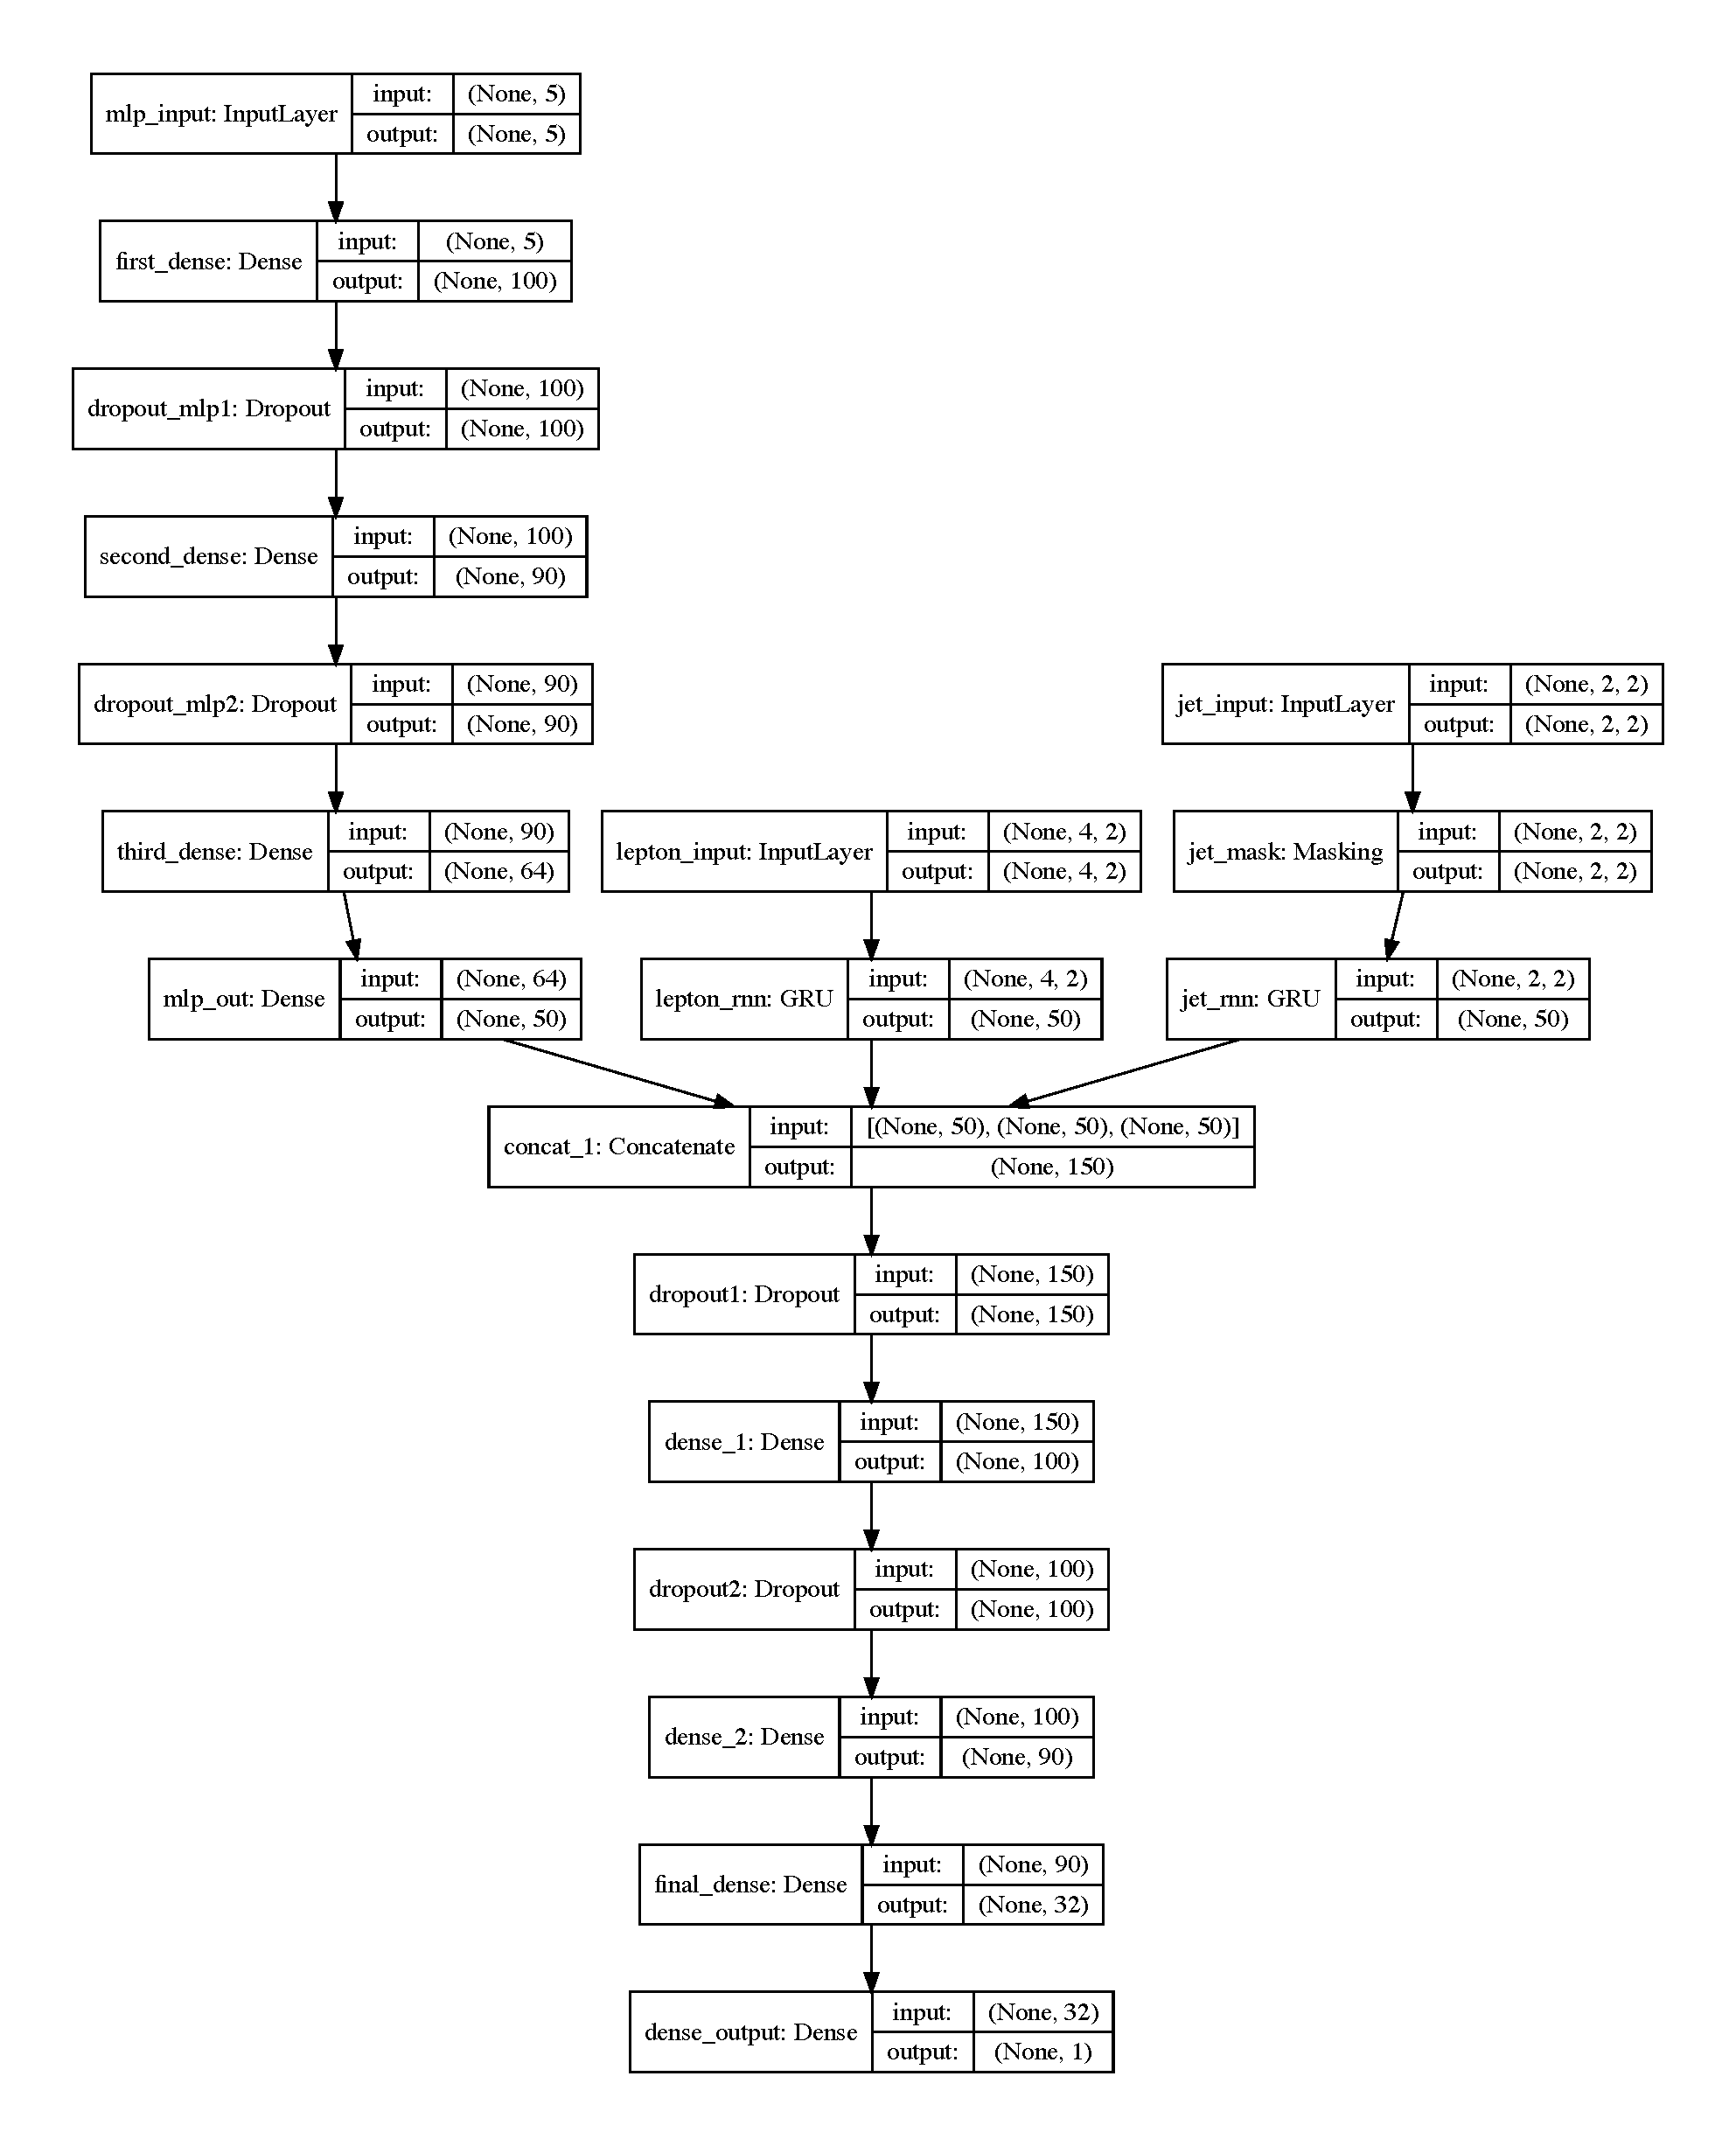
\includegraphics[width=0.49\textwidth]{figures/HMHZZ/selection/model_vbf_architecture.pdf}}
        \subfloat[]{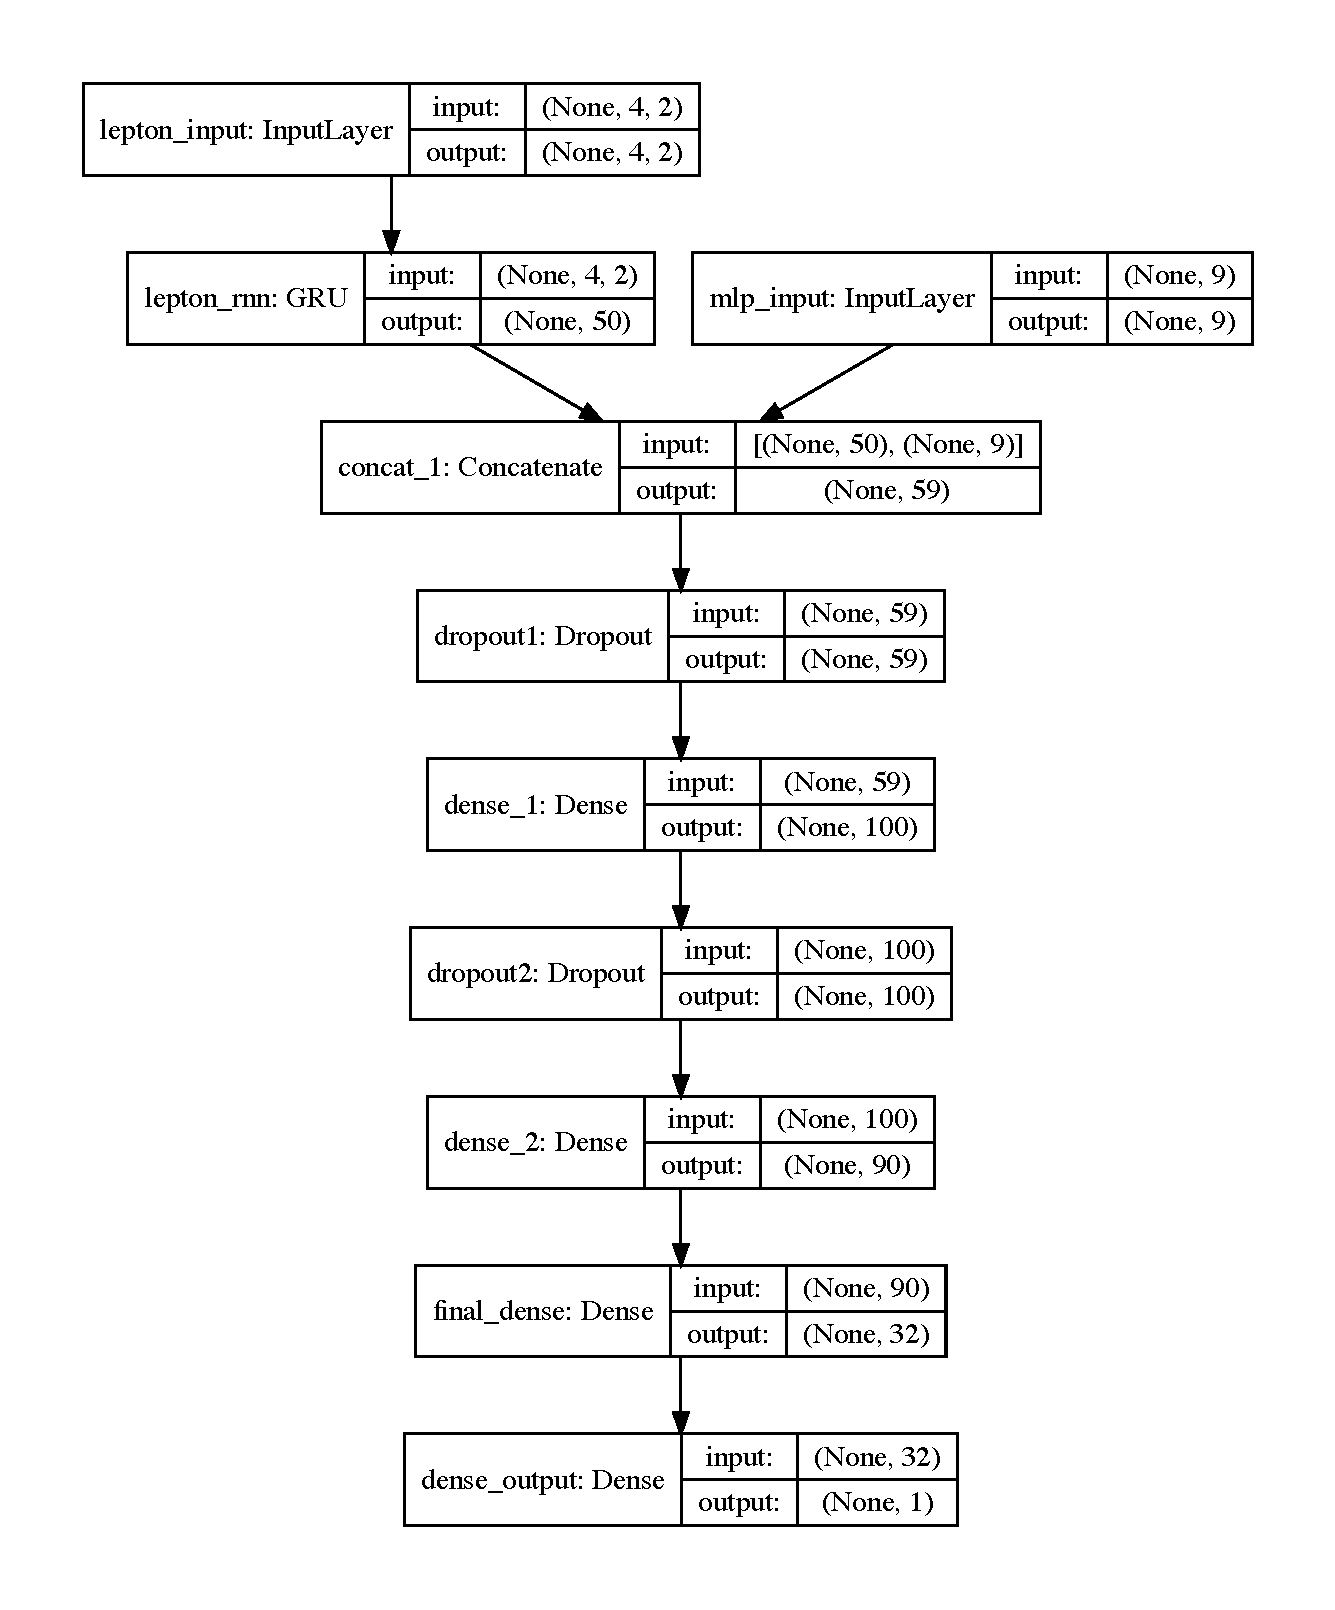
\includegraphics[width=0.49\textwidth]{figures/HMHZZ/selection/model_ggf_architecture.pdf}}
        \caption{(a) VBF DNN architecture diagram. (b) ggF DNN architecture.}
        \label{fig:dnn_arch}
\end{figure}

For training, the VBF and ggF signal samples at the masses of 200, 300, 400, 500, 600, 700, 800, 900, 1000, 1200, 1400~\gev are used with positive label.
The VBF (ggF) signals are only used for VBF (ggF) classifier.
The background (with negative labels) uses simulated samples of QCD and EW \qqZZ processes as well as \ggZZ process summed according to their cross section.
In addition to the selections described in section~\ref{sec:hmhzz_eventsel}, the events used for VBF network are required to have $N_\mathrm{jets} \geq 2$, while $N_\mathrm{jets} < 2$ is required to events for ggF network.

In order to assign equivalent importance to signals and background, during the training, signal events are reweighted to follow the \mfl distribution from background, as shown in figure~\ref{fig:dnn_rwt_vbf} (figure~\ref{fig:dnn_rwt_ggf}) before (left) and after(right) reweighting for VBF (ggF) samples.

\begin{figure}[htbp]
        \centering
        \subfloat[]{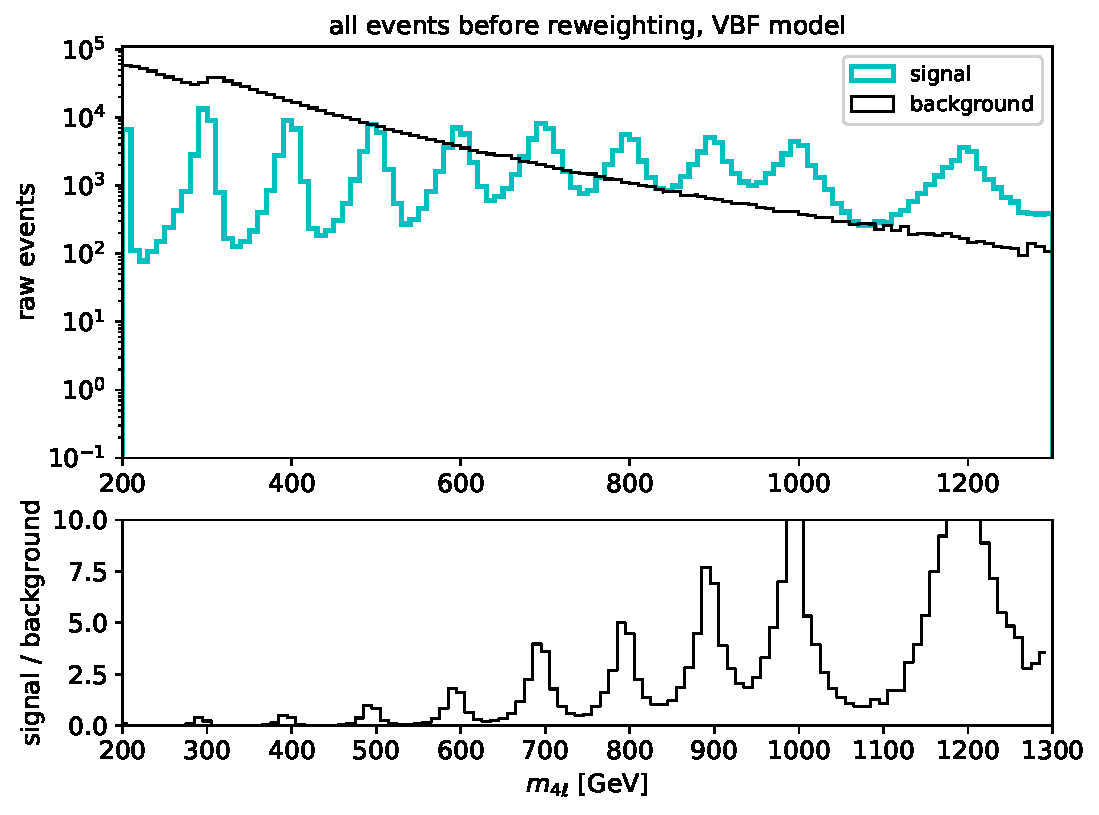
\includegraphics[width=0.48\textwidth]{{figures/HMHZZ/selection/vbf_input/m4l_before_reweighting.pdf}}}
        \subfloat[]{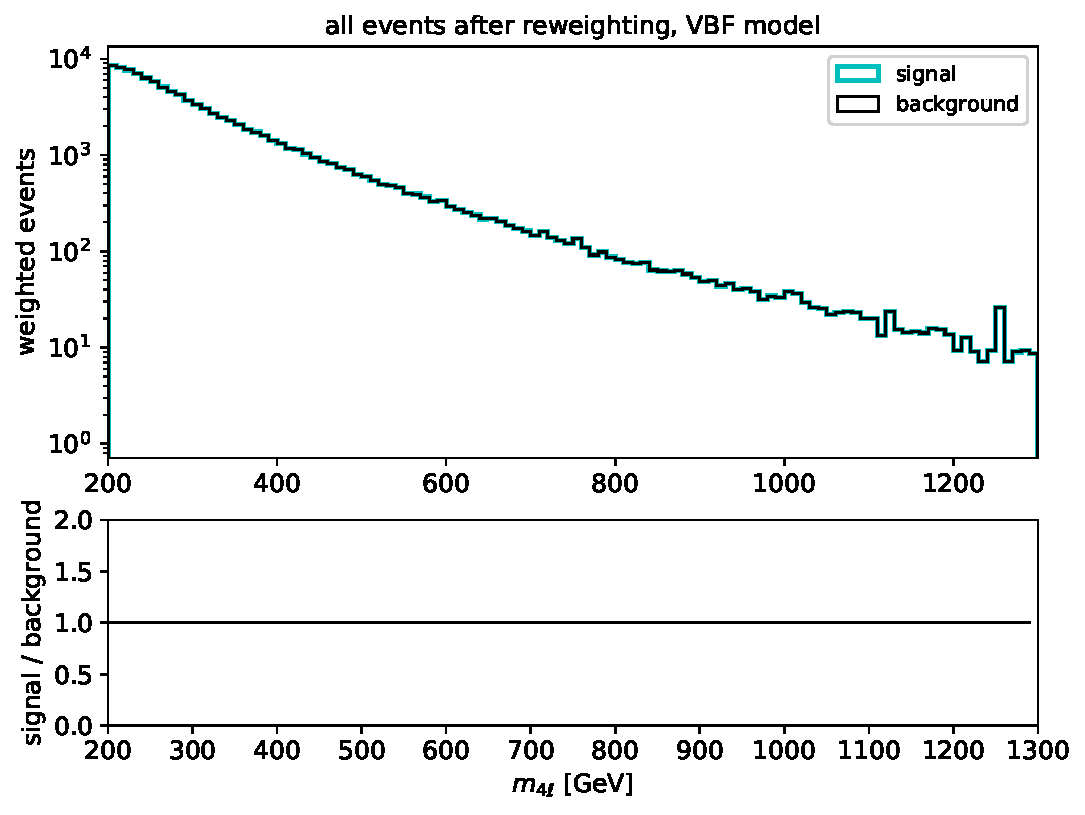
\includegraphics[width=0.48\textwidth]{{figures/HMHZZ/selection/vbf_input/m4l_after_reweighting.pdf}}}
        \caption{(a) \mfl distribution of raw (unweighted) training events for VBF signal (blue) and background (black); (b) \mfl distribution of weighted VBF signal (blue) and background (black) used at training time.}
        \label{fig:dnn_rwt_vbf}
\end{figure}

\begin{figure}[htbp]
        \centering
        \subfloat[]{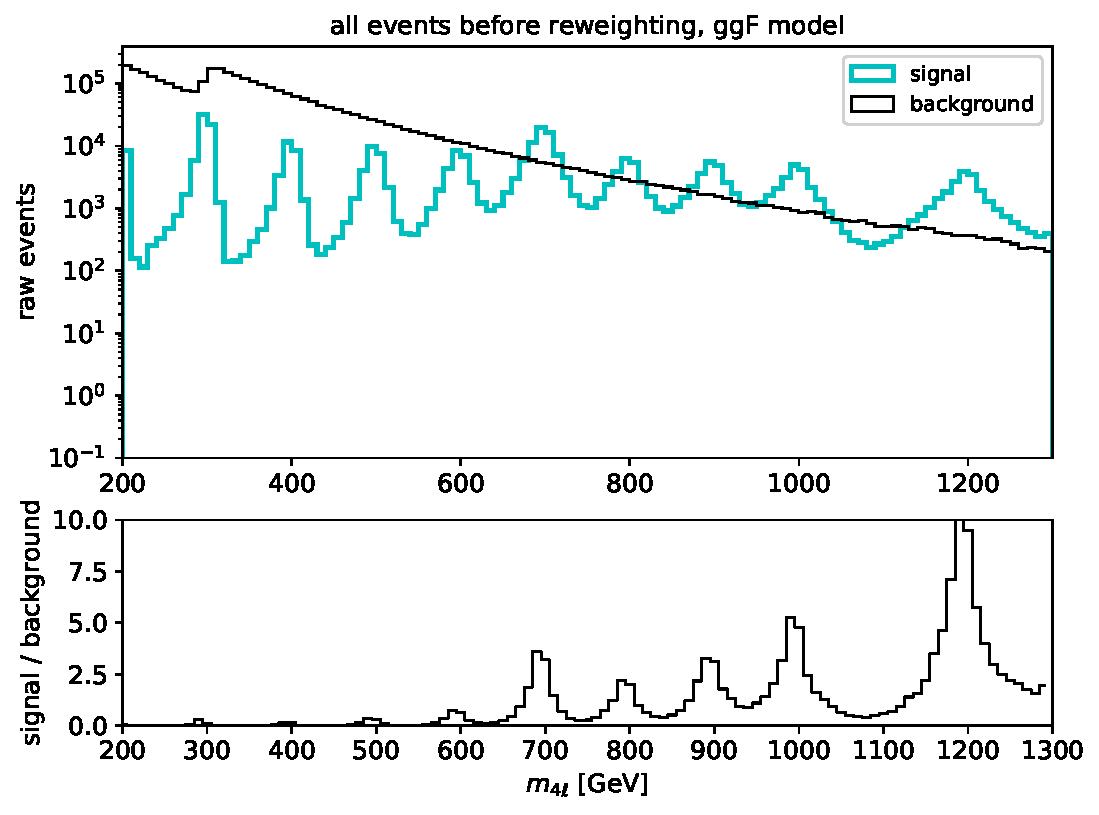
\includegraphics[width=0.48\textwidth]{{figures/HMHZZ/selection/ggf_input/m4l_all_before_reweighting.pdf}}}
        \subfloat[]{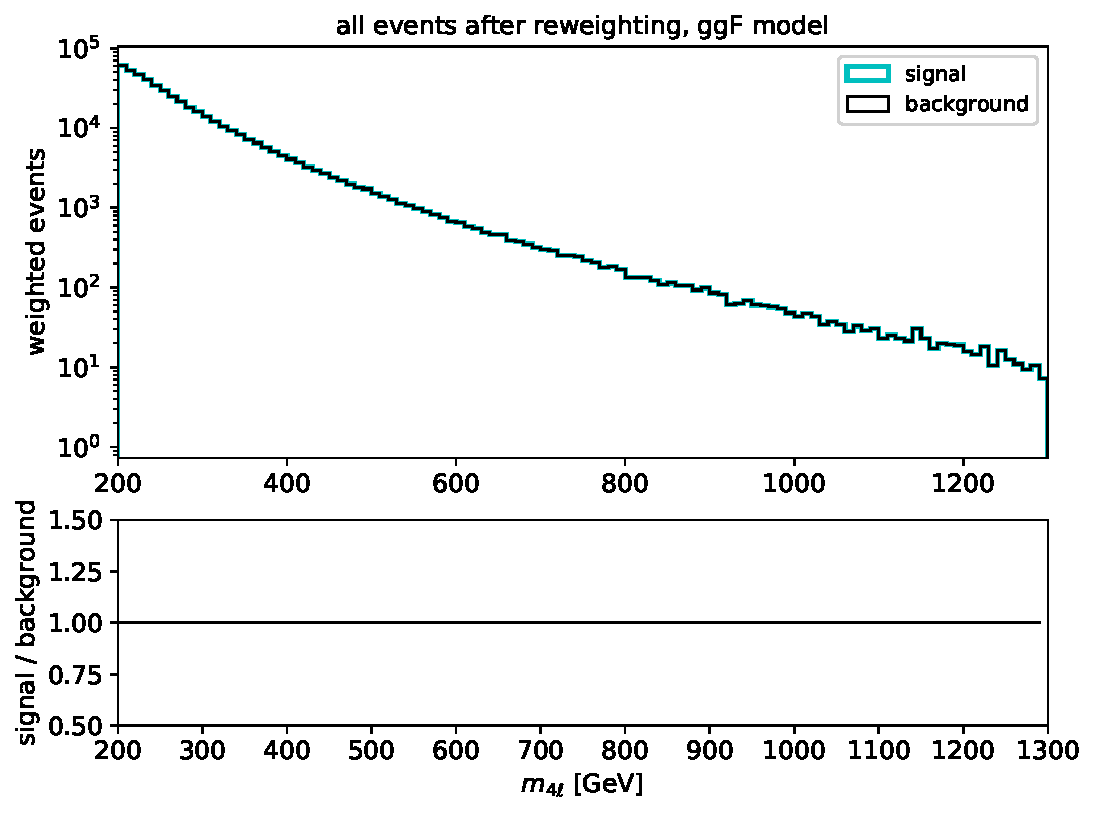
\includegraphics[width=0.48\textwidth]{{figures/HMHZZ/selection/ggf_input/m4l_all_after_reweighting.pdf}}}
        \caption{(a) \mfl distribution of raw (unweighted) training events for ggF signal (blue) and background (black); (b) \mfl distribution of weighted ggF signal (blue) and background (black) used at training time.}
        \label{fig:dnn_rwt_ggf}
\end{figure}

%After all these preparation, then the training is performed over 20 epochs with batch size of 512 (256) for VBF (ggF) network.


\textbf{Input features} \\
Table~\ref{tab:dnn_features_vbf} (table~\ref{tab:dnn_features_ggf}) lists the input features used for VBF (ggF) network during the training.
For VBF network, one RNN (the other one) takes the \pt and \eta of \pt-ordered four leptons (two leading jets) as input features, which intends to study the time relationship from particle decay between leptons (jets).
For ggF network, the only one RNN model takes as input features of the \pt and \eta of \pt-ordered four leptons.

\begin{table}[htbp]
        \centering
        \caption{Input features for the VBF network.}
        \label{tab:dnn_features_vbf}
        \begin{tabular}{c | c}
                \toprule
                Variable & Description \\
                \midrule
                $m_{4\ell}$ & 4$\ell$ invariant mass \\
                $m_{jj}$ & dijet invariant mass \\
                $p_\mathrm{T}^{jj}$ & dijet transverse momentum\\
                $\Delta\eta_{H,j}$ & difference in pseudorapidities between the 4$\ell$ system and the leading jet \\
                $\min \Delta R _{jZ}$ & minimum angular separation between one of the two $\ell\ell$ pairs and a jet\\
                $p_\mathrm{T}^j$ & transverse momenta of the two leading jets \\
                $\eta^j$ & pseudorapidities of the two leading jets \\
                $p_\mathrm{T}^\ell$ & transverse momenta of the four leptons \\
                $\eta^\ell$ & pseudorapidities of the four leptons  \\
                \bottomrule
        \end{tabular}
\end{table}

\begin{table}[htbp]
        \centering
        \caption{Input features for the ggF network.}
        \label{tab:dnn_features_ggf}
        \begin{tabular}{c | c}
                \toprule
                Variable & Description \\
                \midrule
                $m_{4\ell}$ & 4$\ell$ invariant mass \\
                $\cos\theta_1$ & decay angle of the leading $Z$ \\
                $\cos\theta_2$ & decay angle of the sub-leading $Z$ \\
                $\cos\theta^*$ & production angle of the $ZZ$ system \\
                $\Delta R _{jH}$ & angular separation between the 4$\ell$ system and the leading jet\\
                $\phi$ & azimuthal angle of the $ZZ$ system \\
                $p_\mathrm{T}^{4\ell}$ & transverse momentum of the $4\ell$ system \\
                $\eta^{4\ell}$ & pseudorapidity of the $4\ell$ system \\
                $p_\mathrm{T}^j$ & transverse momentum of up to one jet \\
                $\eta^j$ & pseudorapidity of up to one jet \\
                $p_\mathrm{T}^\ell$ & transverse momenta of the four leptons \\
                $\eta^\ell$ & pseudorapidities of the four leptons  \\
                \bottomrule
        \end{tabular}
\end{table}

%Figure~\ref{fig:dnn_vbf_distribution} (figure~\ref{fig:dnn_ggf_distribution}) shows the distributions of input features with events before training reweighting for VBF (ggF) network of background and 4 signal samples at mass points of 300, 700, 1400 and 2000~\gev.
%
%\begin{figure}[htbp]
%        \captionsetup[subfigure]{labelformat=empty}
%        \centering
%        \subfloat[]{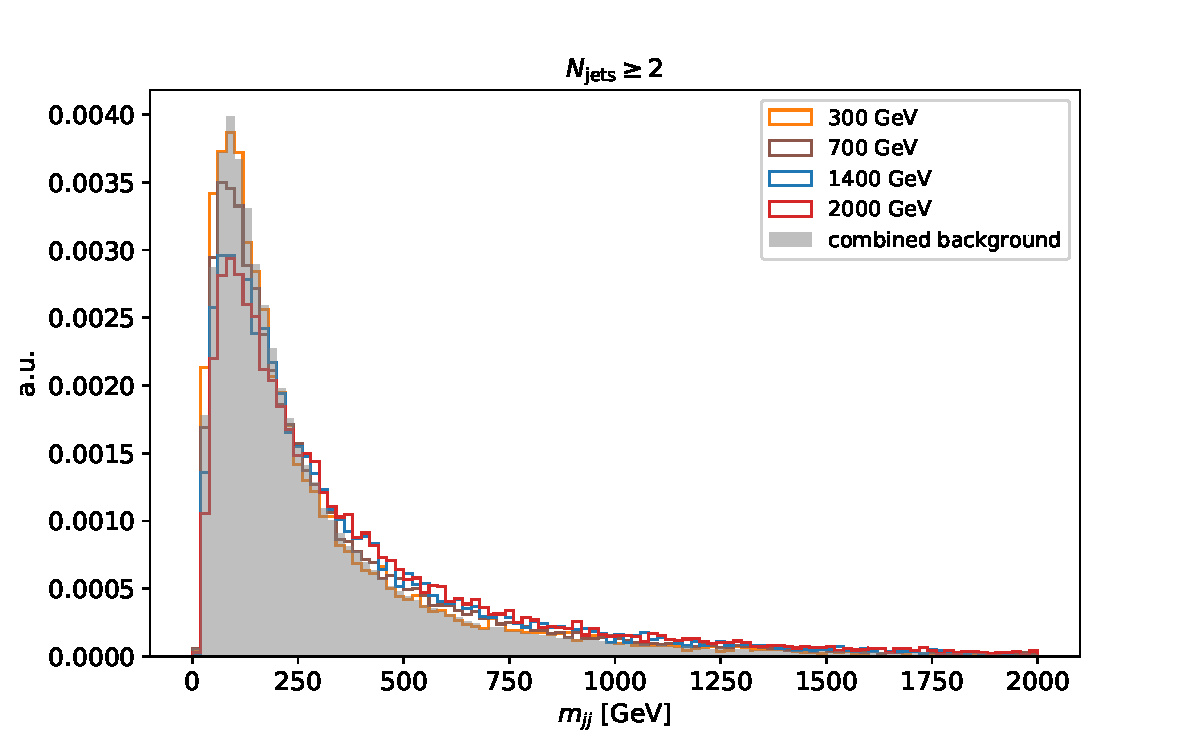
\includegraphics[width=0.19\textwidth]{figures/HMHZZ/selection/vbf_input/input_comparison_300_to_2000_0_score_dijet_invmass}}
%        \subfloat[]{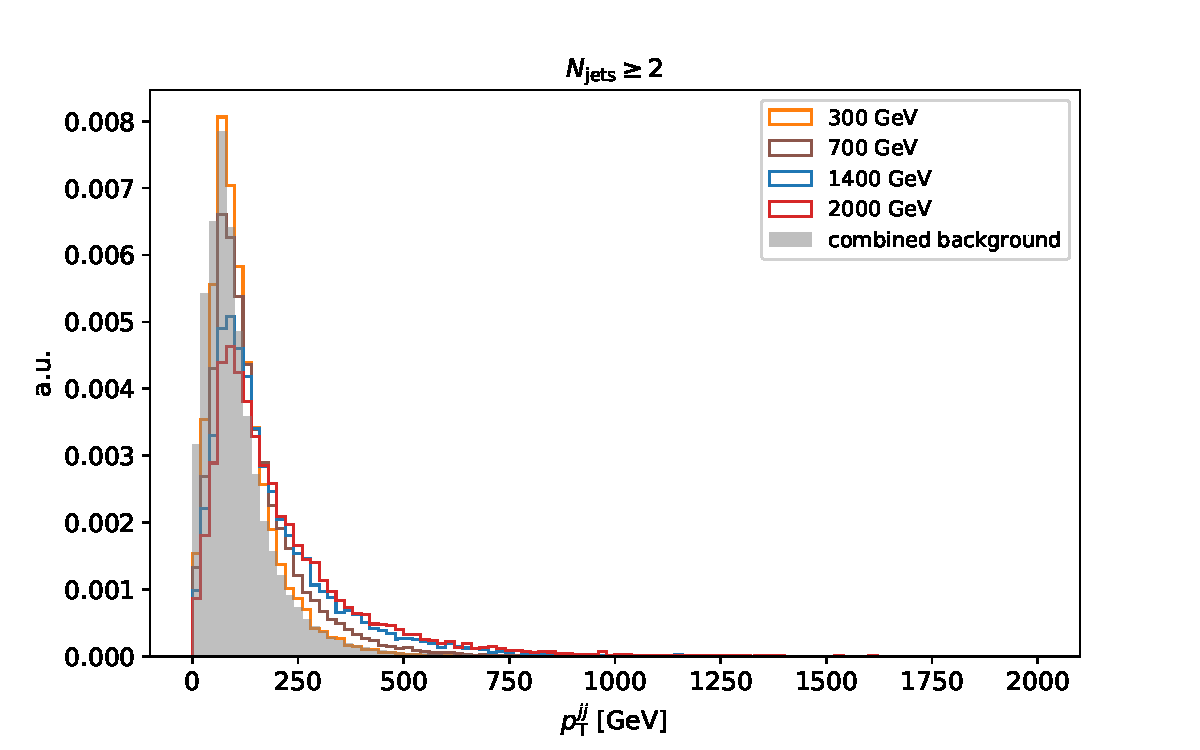
\includegraphics[width=0.19\textwidth]{figures/HMHZZ/selection/vbf_input/input_comparison_300_to_2000_2_score_dijet_pt}}
%        \subfloat[]{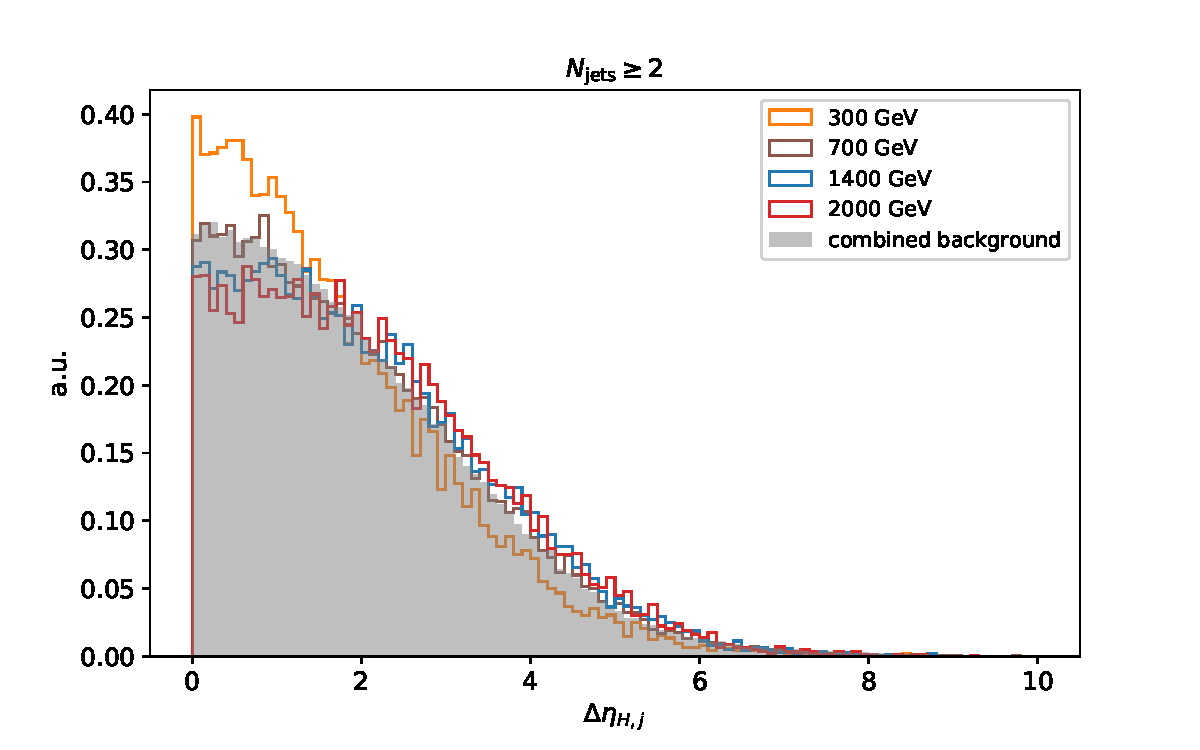
\includegraphics[width=0.19\textwidth]{figures/HMHZZ/selection/vbf_input/input_comparison_300_to_2000_3_score_eta_zepp_ZZ}}
%        \subfloat[]{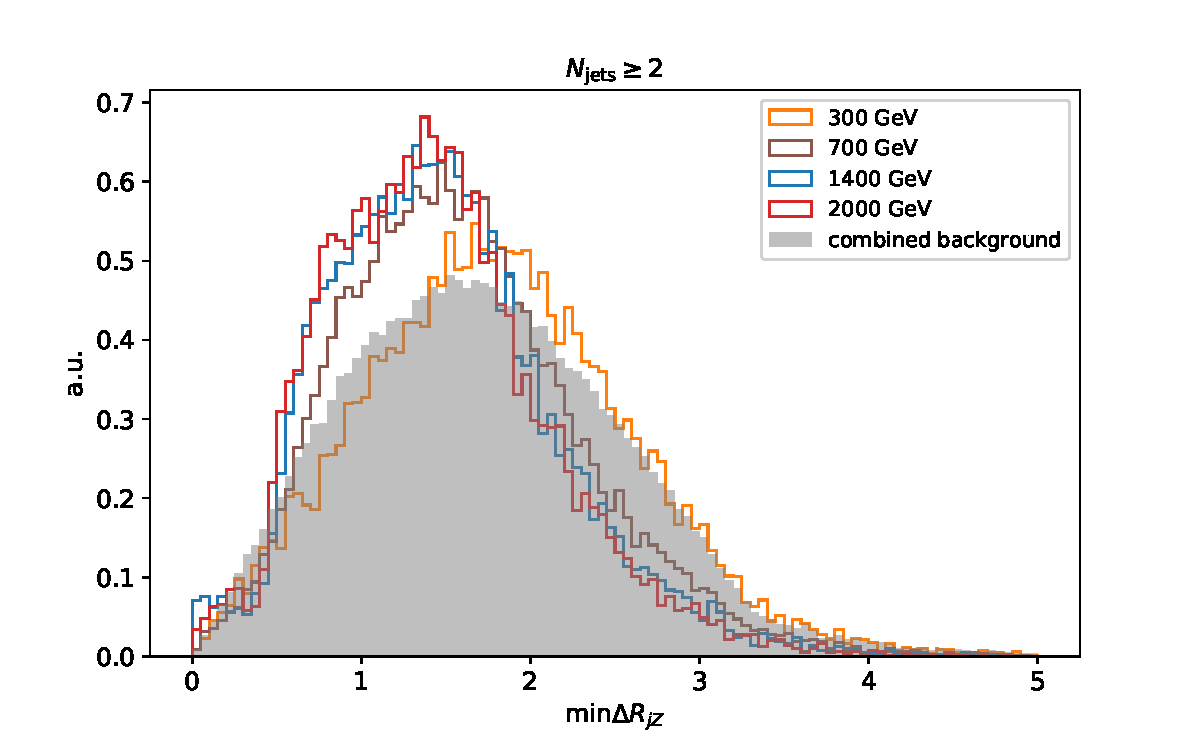
\includegraphics[width=0.19\textwidth]{figures/HMHZZ/selection/vbf_input/input_comparison_300_to_2000_4_score_min_dR_jZ}}
%        \subfloat[]{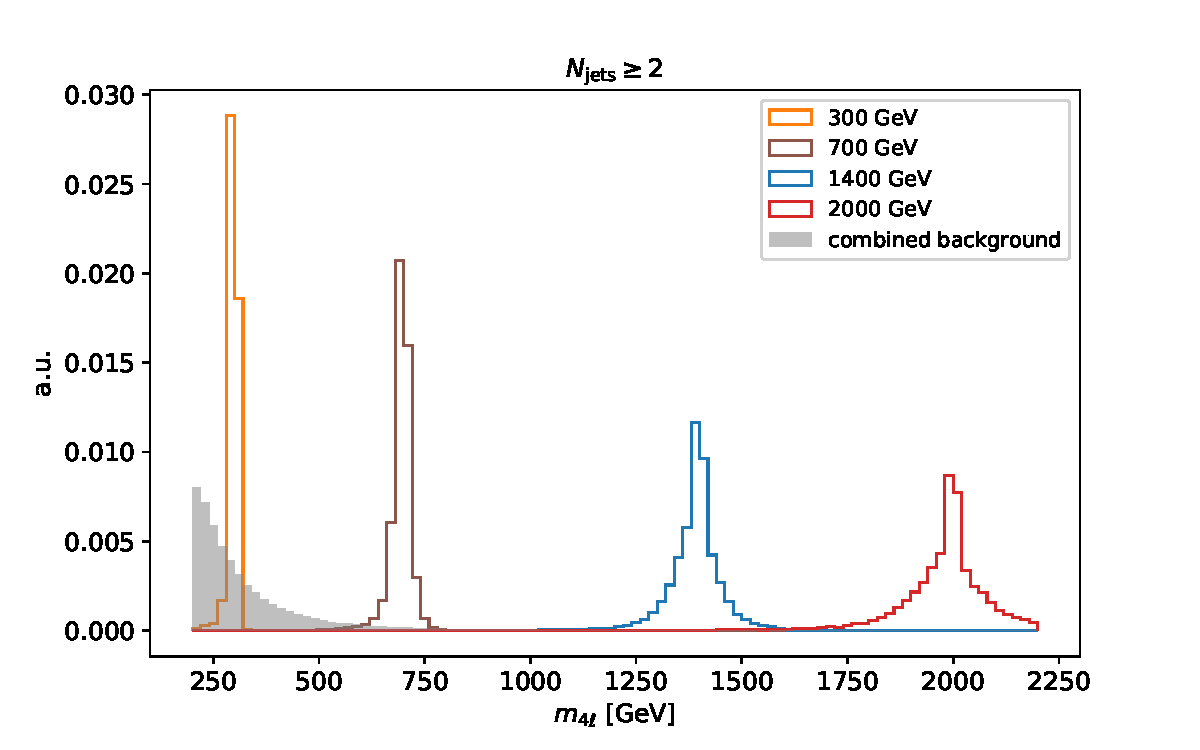
\includegraphics[width=0.19\textwidth]{figures/HMHZZ/selection/vbf_input/input_comparison_300_to_2000_5_score_m4l_unconstrained}}\\
%
%        \subfloat[]{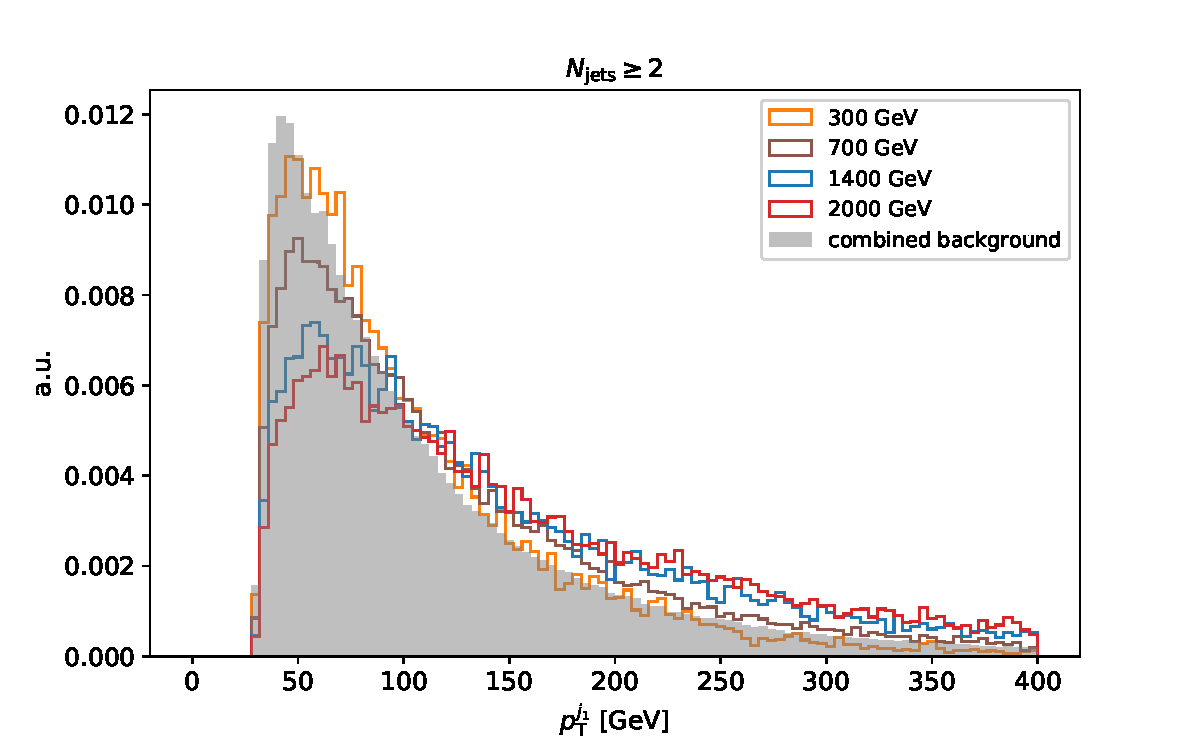
\includegraphics[width=0.24\textwidth]{figures/HMHZZ/selection/vbf_input/input_comparison_300_to_2000_23_score_j_1_pt}}
%        \subfloat[]{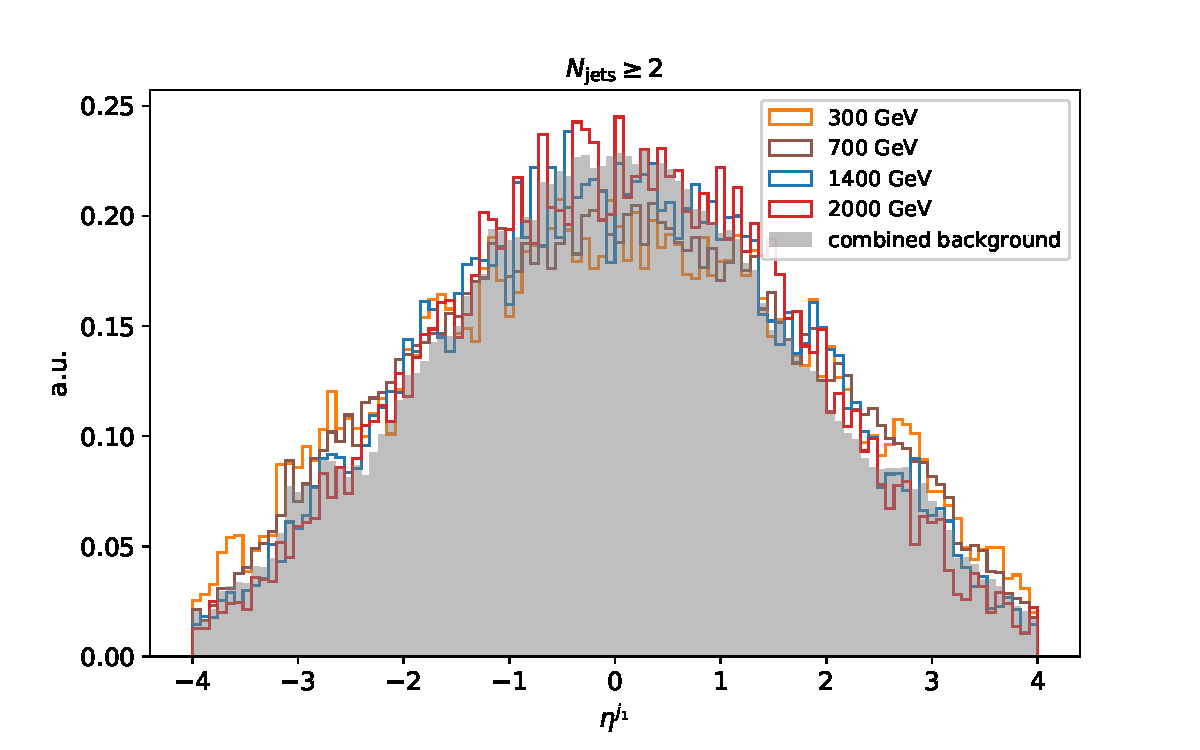
\includegraphics[width=0.24\textwidth]{figures/HMHZZ/selection/vbf_input/input_comparison_300_to_2000_24_score_j_1_eta}}
%        \subfloat[]{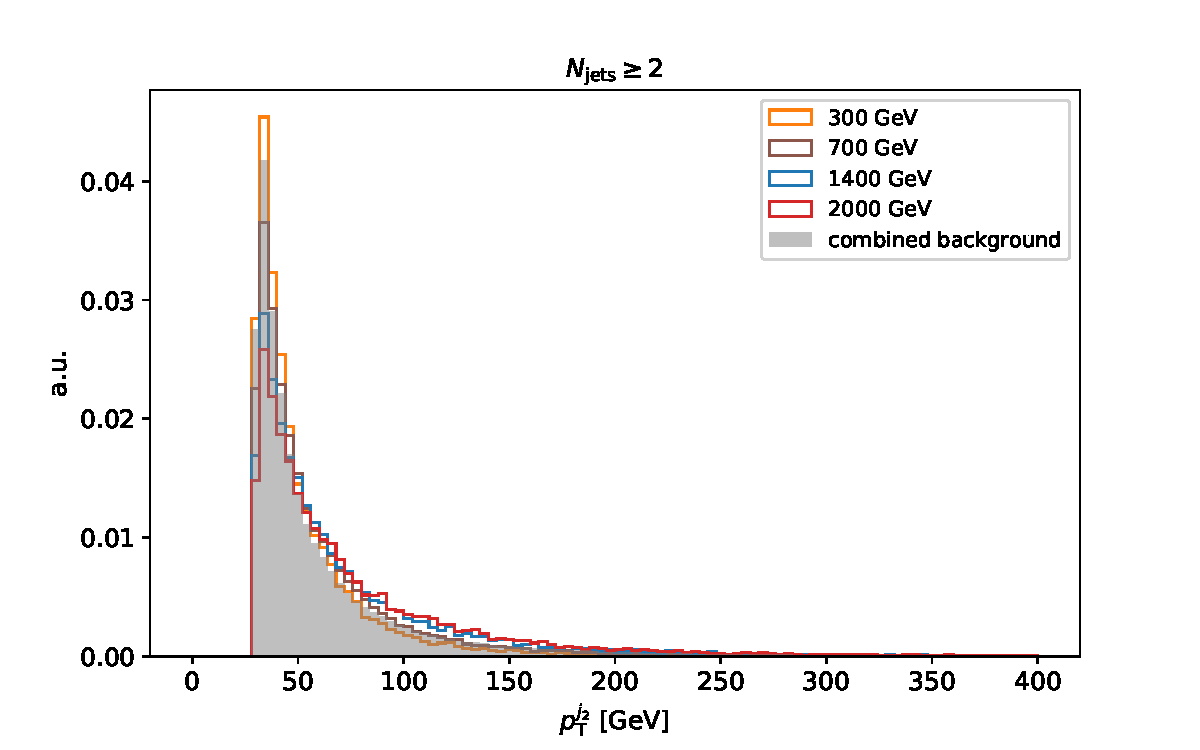
\includegraphics[width=0.24\textwidth]{figures/HMHZZ/selection/vbf_input/input_comparison_300_to_2000_25_score_j_2_pt}}
%        \subfloat[]{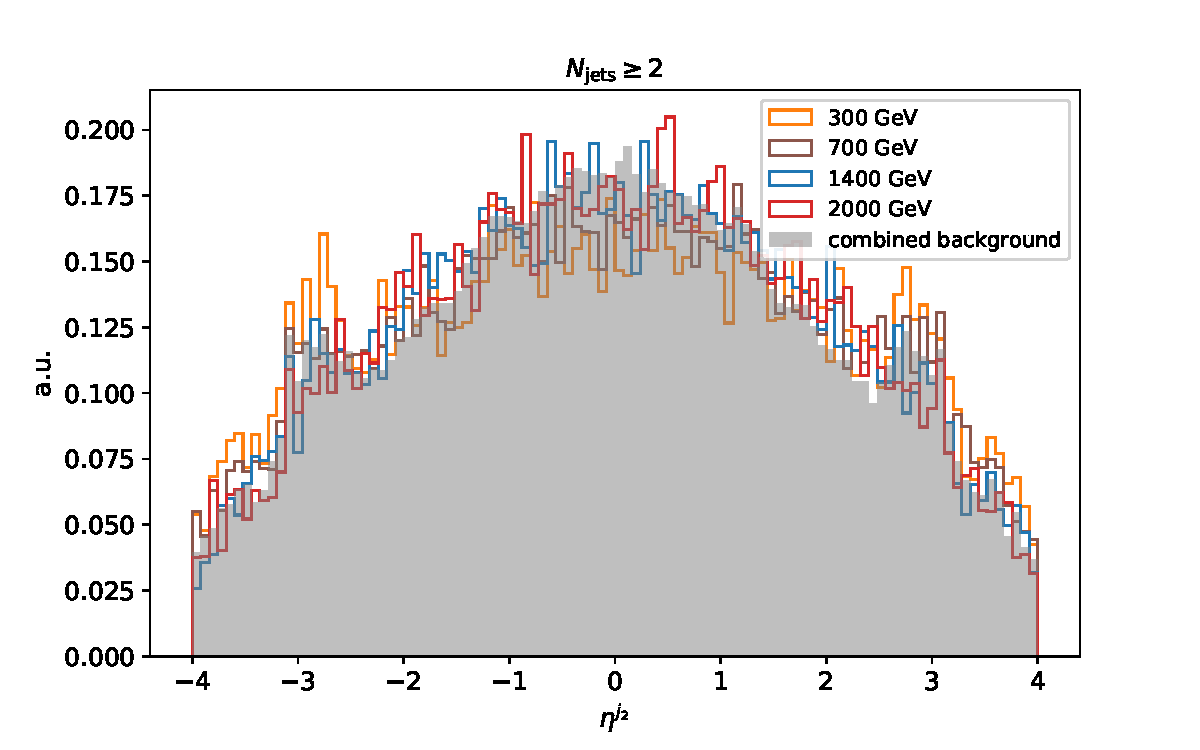
\includegraphics[width=0.24\textwidth]{figures/HMHZZ/selection/vbf_input/input_comparison_300_to_2000_26_score_j_2_eta}}\\
%
%        \subfloat[]{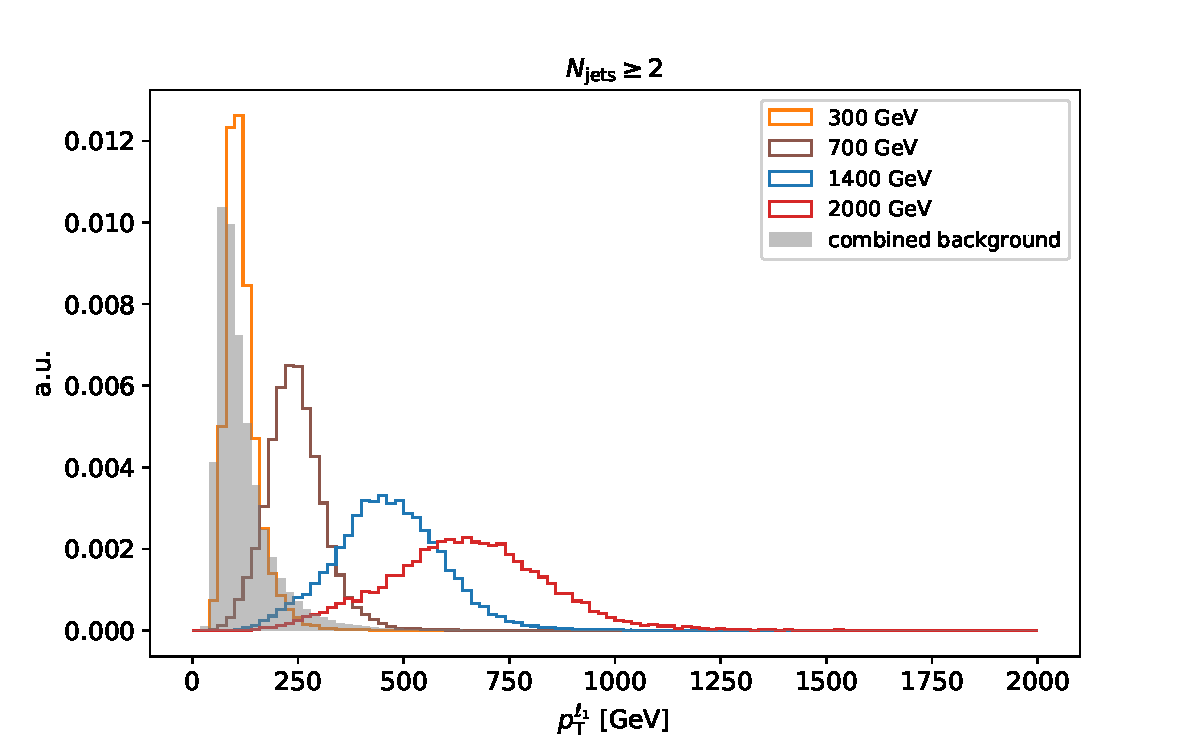
\includegraphics[width=0.24\textwidth]{figures/HMHZZ/selection/vbf_input/input_comparison_300_to_2000_15_score_lep_1_pt}}
%        \subfloat[]{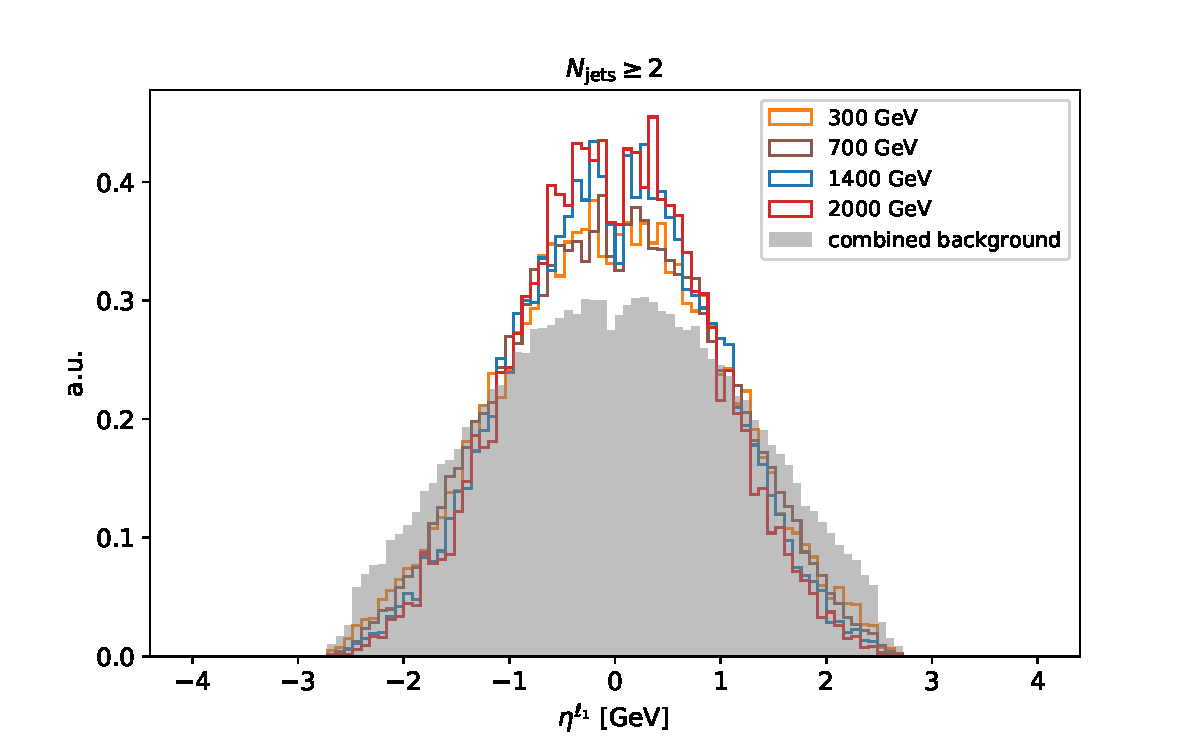
\includegraphics[width=0.24\textwidth]{figures/HMHZZ/selection/vbf_input/input_comparison_300_to_2000_16_score_lep_1_eta}}
%        \subfloat[]{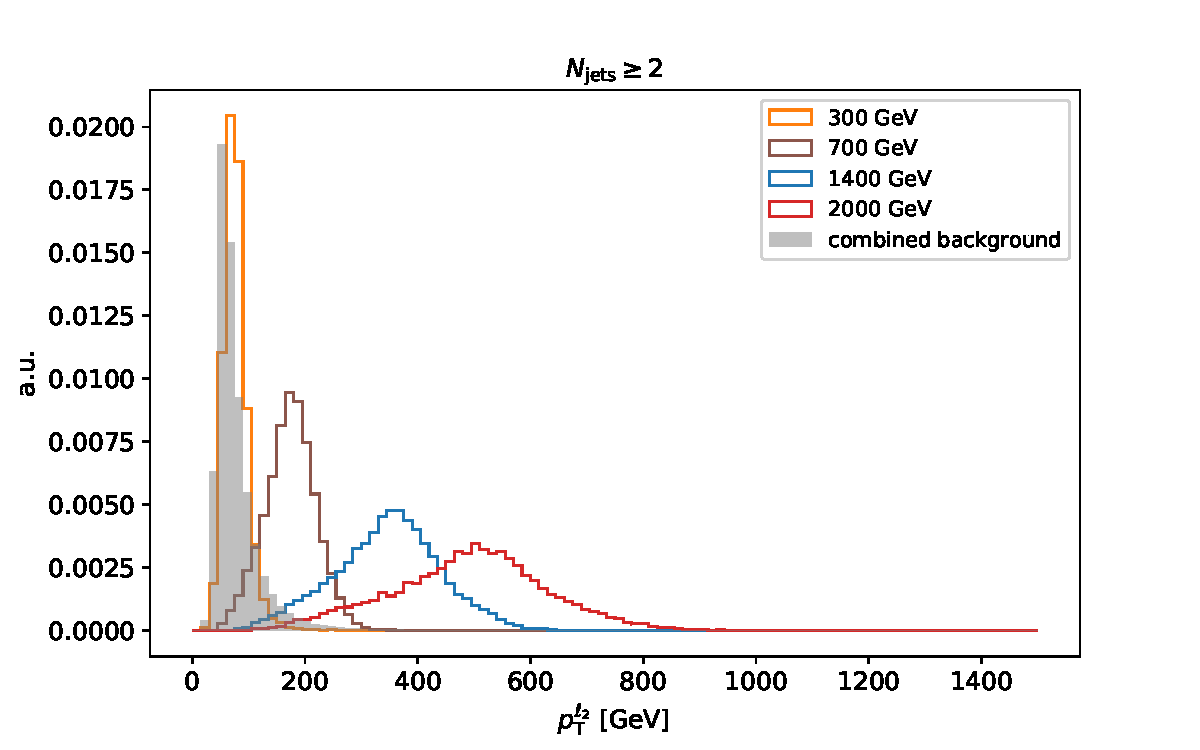
\includegraphics[width=0.24\textwidth]{figures/HMHZZ/selection/vbf_input/input_comparison_300_to_2000_17_score_lep_2_pt}}
%        \subfloat[]{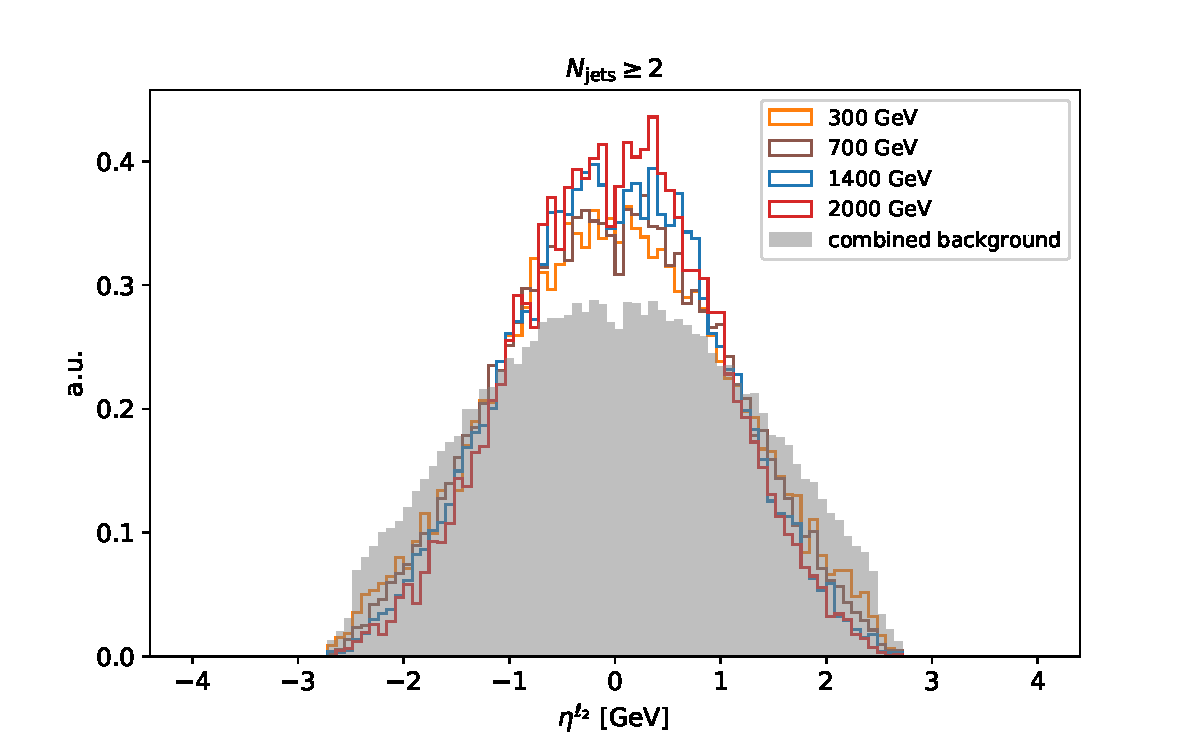
\includegraphics[width=0.24\textwidth]{figures/HMHZZ/selection/vbf_input/input_comparison_300_to_2000_18_score_lep_2_eta}}\\
%
%        \subfloat[]{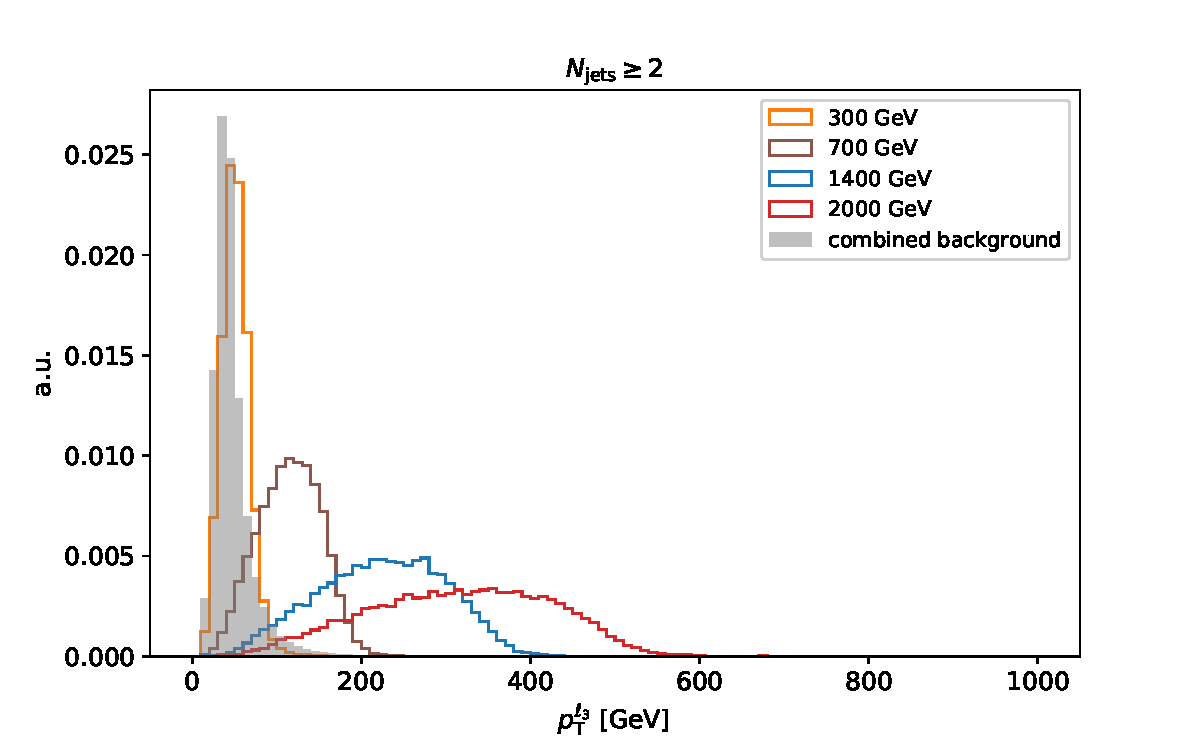
\includegraphics[width=0.24\textwidth]{figures/HMHZZ/selection/vbf_input/input_comparison_300_to_2000_19_score_lep_3_pt}}
%        \subfloat[]{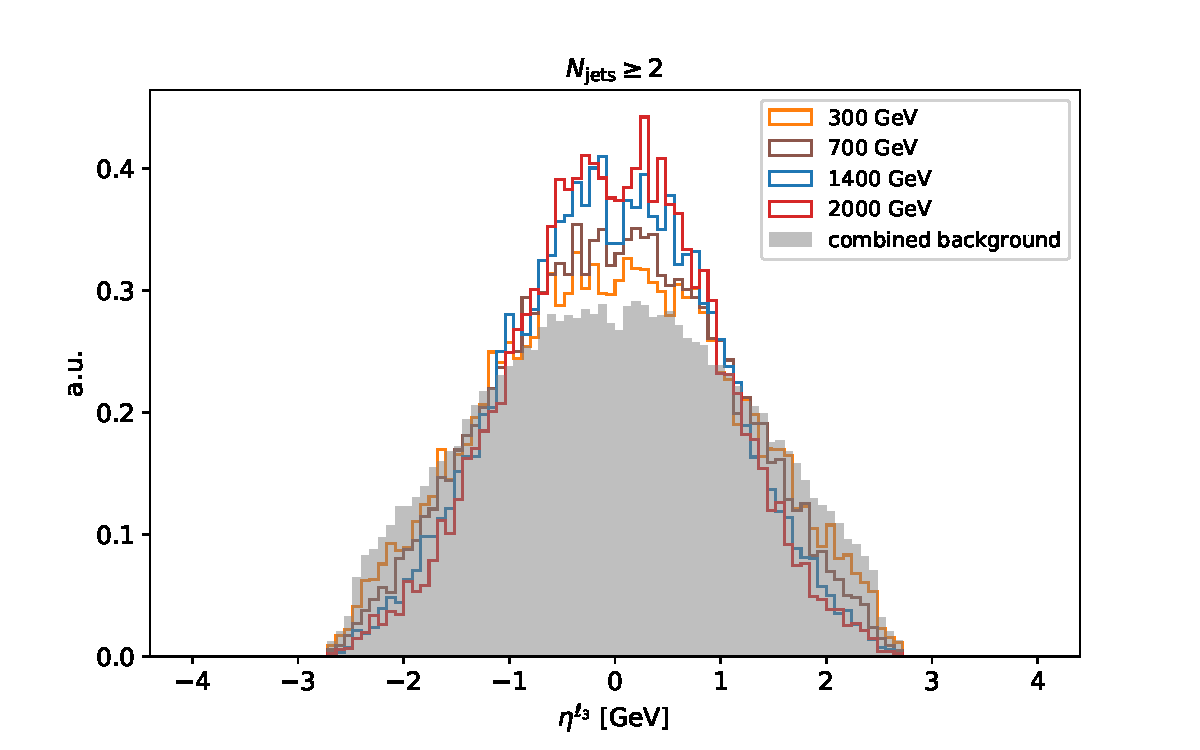
\includegraphics[width=0.24\textwidth]{figures/HMHZZ/selection/vbf_input/input_comparison_300_to_2000_20_score_lep_3_eta}}
%        \subfloat[]{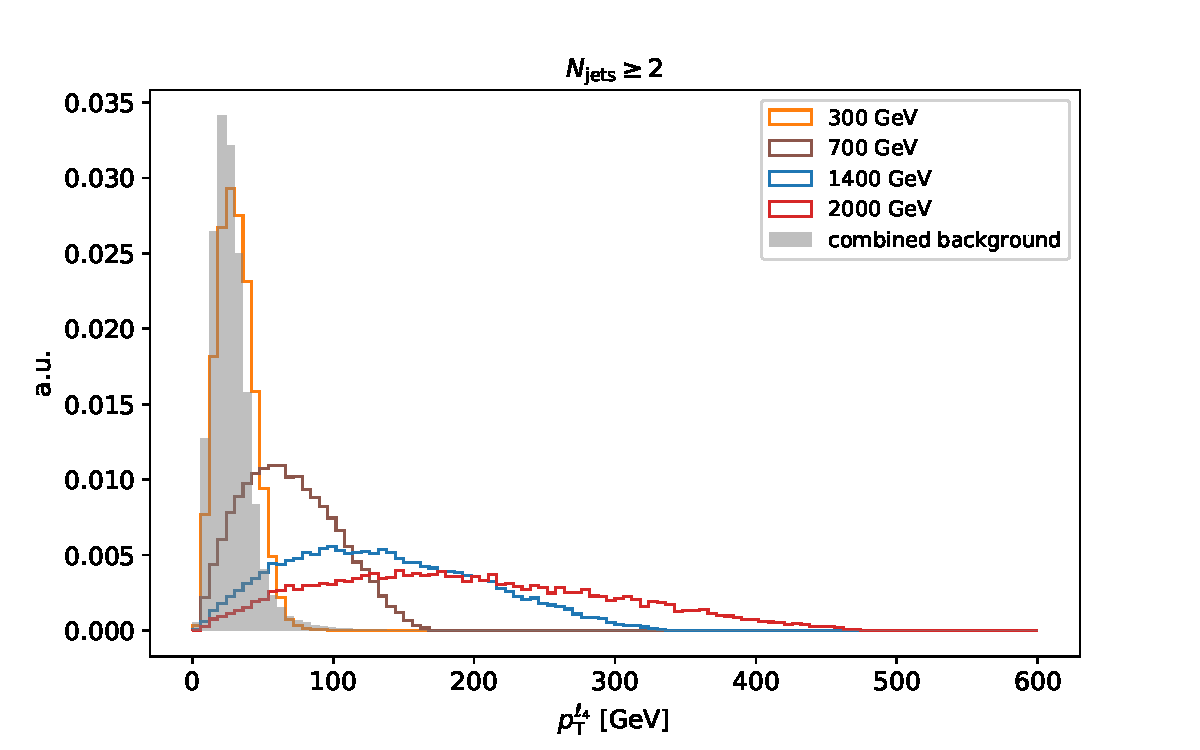
\includegraphics[width=0.24\textwidth]{figures/HMHZZ/selection/vbf_input/input_comparison_300_to_2000_21_score_lep_4_pt}}
%        \subfloat[]{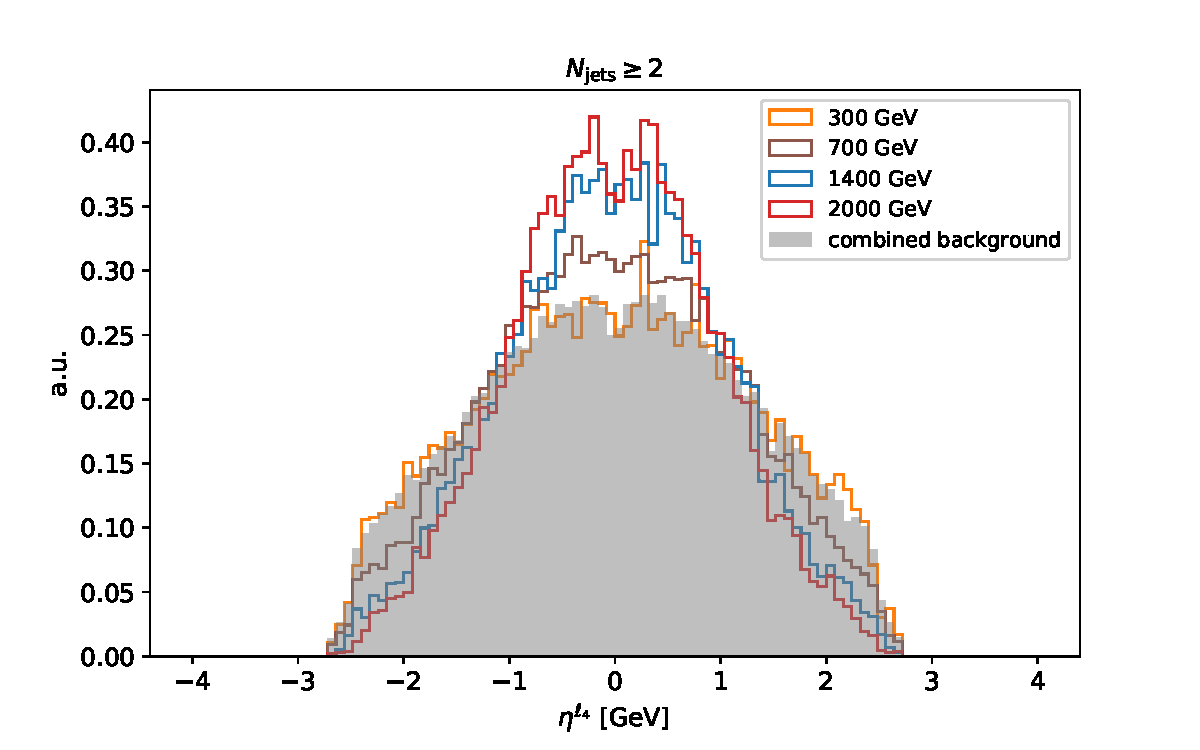
\includegraphics[width=0.24\textwidth]{figures/HMHZZ/selection/vbf_input/input_comparison_300_to_2000_22_score_lep_4_eta}}\\
%        \caption{Distributions of input features as listed in table~\ref{tab:dnn_features_vbf} for the VBF network of signals at mass points of 300, 700, 1400, 2000~\gev (coloured) and the background (grey). Only events satisfying the training selection of $N_\mathrm{jets}\geq2$ are shown.}
%        \label{fig:dnn_vbf_distribution}
%\end{figure}

%\begin{figure}[htbp]
%        \centering
%        \captionsetup[subfigure]{labelformat=empty}
%        \subfloat[]{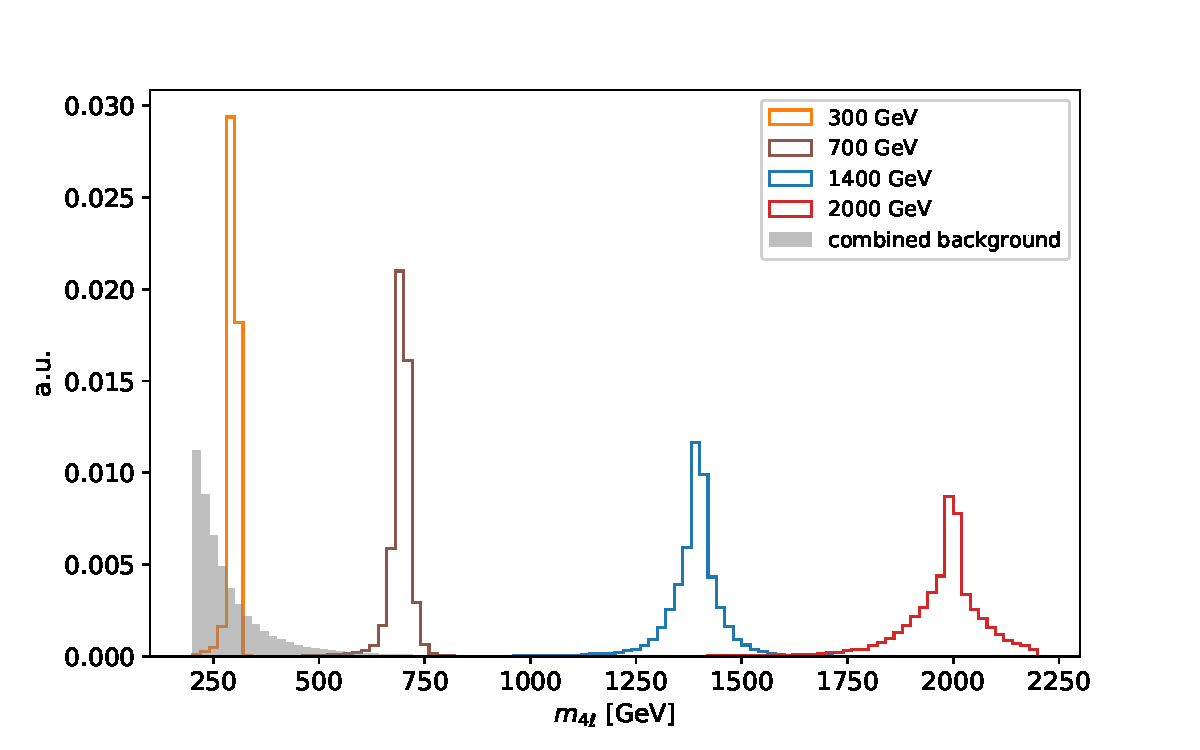
\includegraphics[width=0.24\textwidth]{figures/HMHZZ/selection/ggf_input/input_comparison_300_to_2000_5_score_m4l_unconstrained}}
%        \subfloat[]{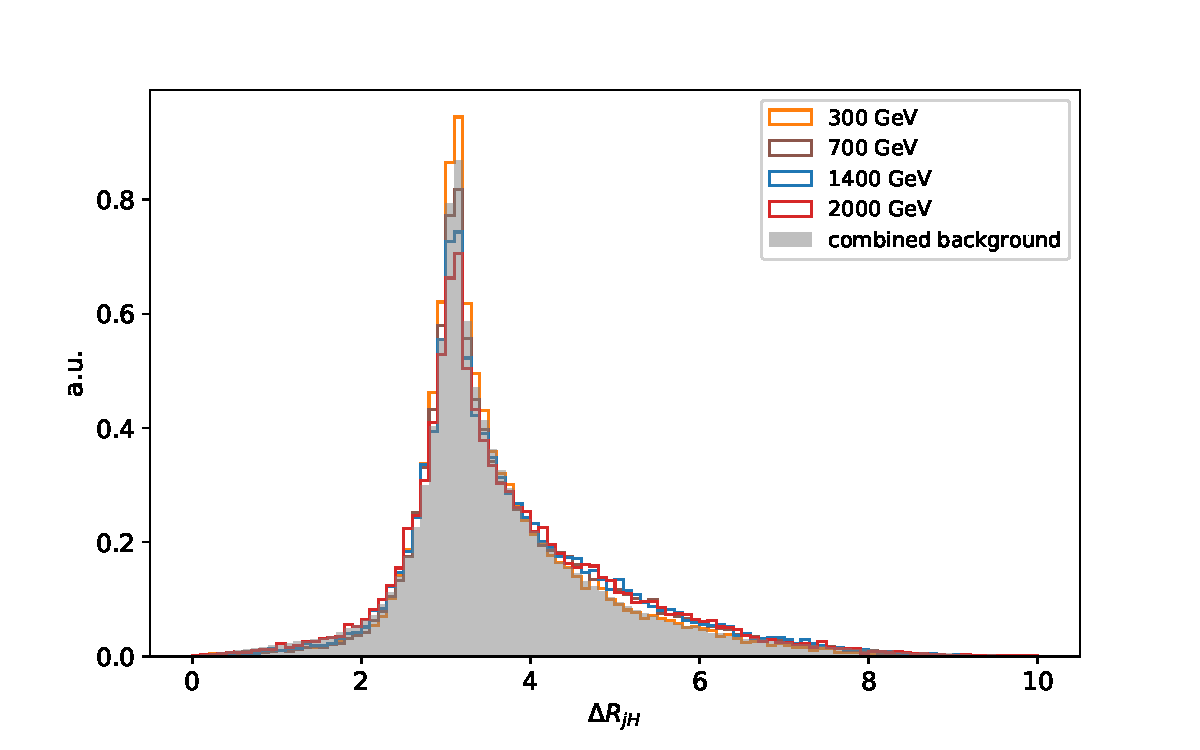
\includegraphics[width=0.24\textwidth]{figures/HMHZZ/selection/ggf_input/input_comparison_300_to_2000_6_score_dR_jH}}
%        \subfloat[]{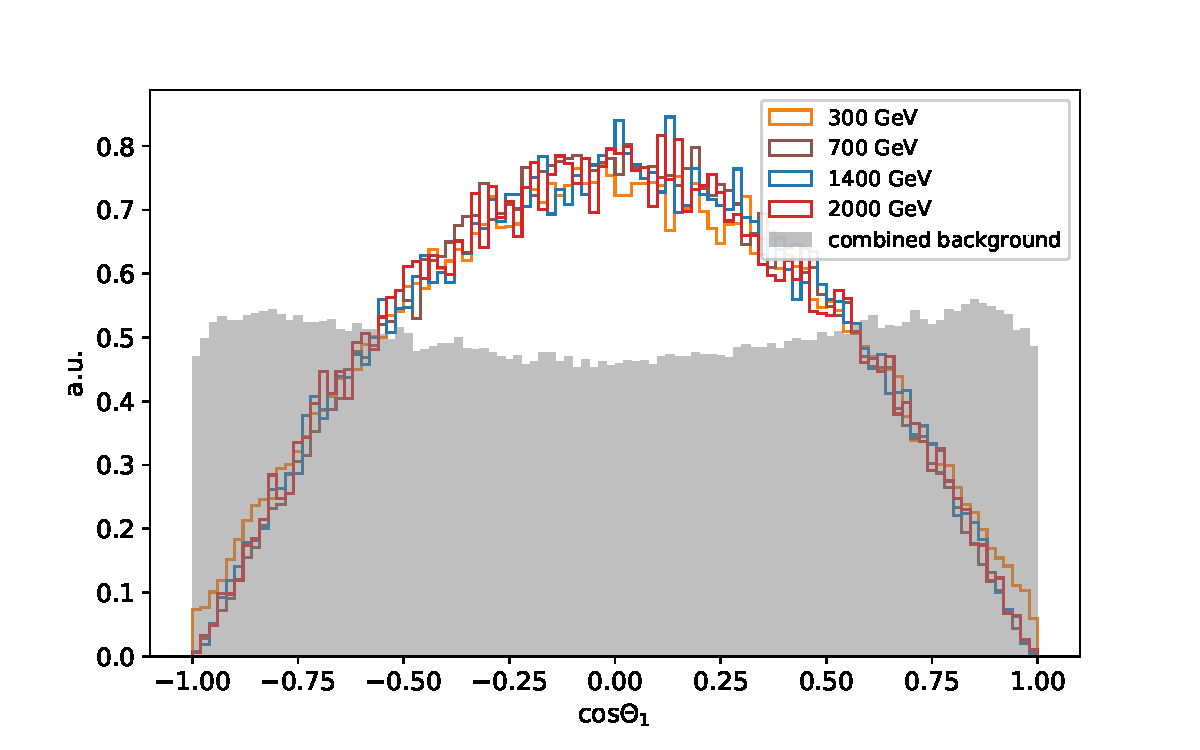
\includegraphics[width=0.24\textwidth]{figures/HMHZZ/selection/ggf_input/input_comparison_300_to_2000_7_score_cth1_unconstrained}}
%        \subfloat[]{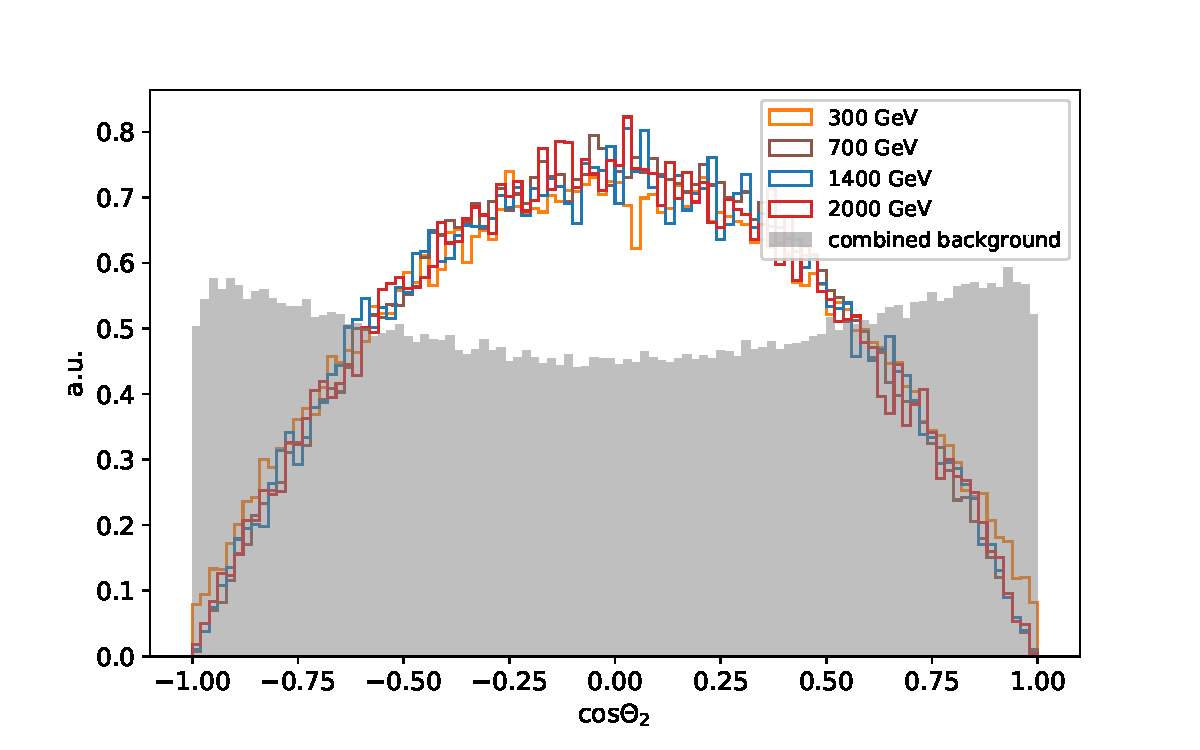
\includegraphics[width=0.24\textwidth]{figures/HMHZZ/selection/ggf_input/input_comparison_300_to_2000_8_score_cth2_unconstrained}}\\
%
%        \subfloat[]{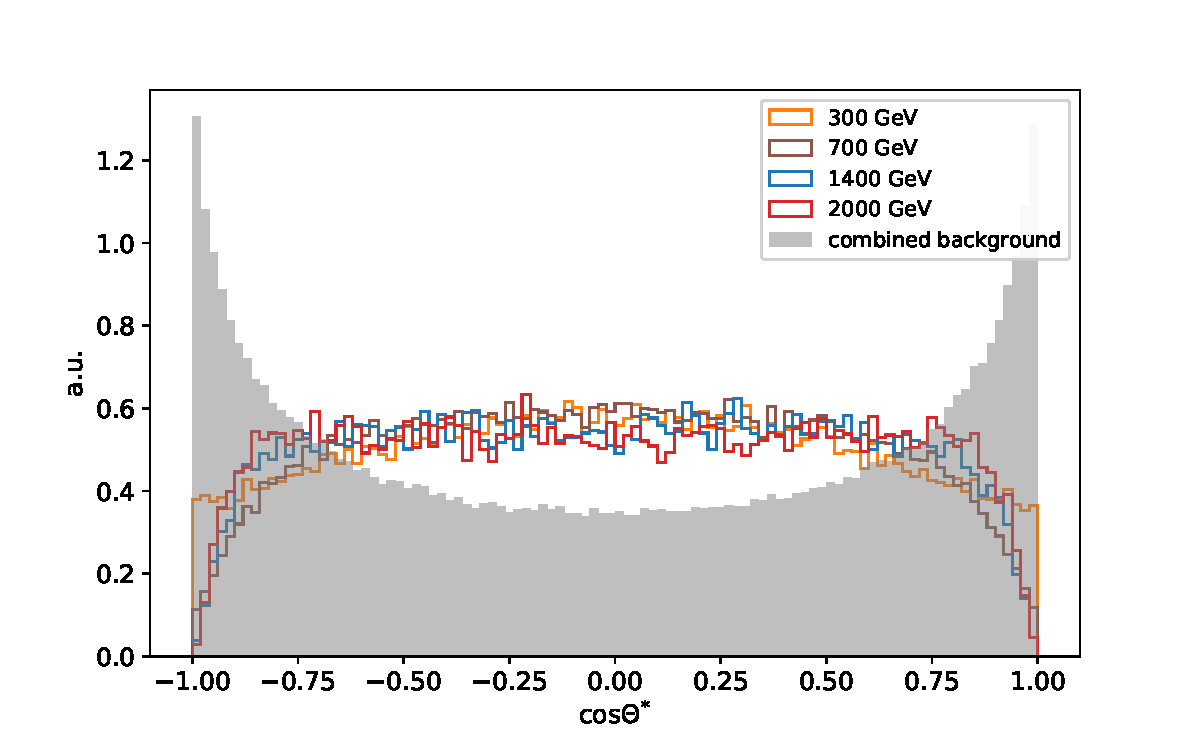
\includegraphics[width=0.24\textwidth]{figures/HMHZZ/selection/ggf_input/input_comparison_300_to_2000_9_score_cthstr_unconstrained}}
%        \subfloat[]{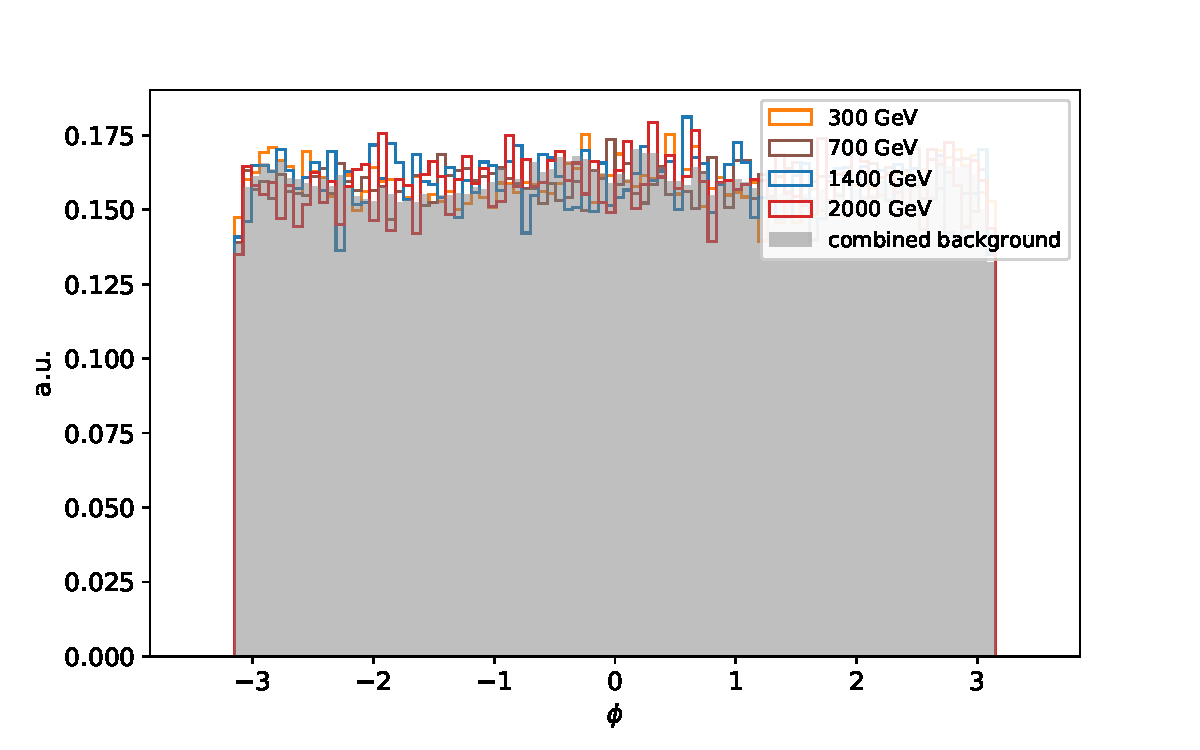
\includegraphics[width=0.24\textwidth]{figures/HMHZZ/selection/ggf_input/input_comparison_300_to_2000_10_score_phi_unconstrained}}
%        \subfloat[]{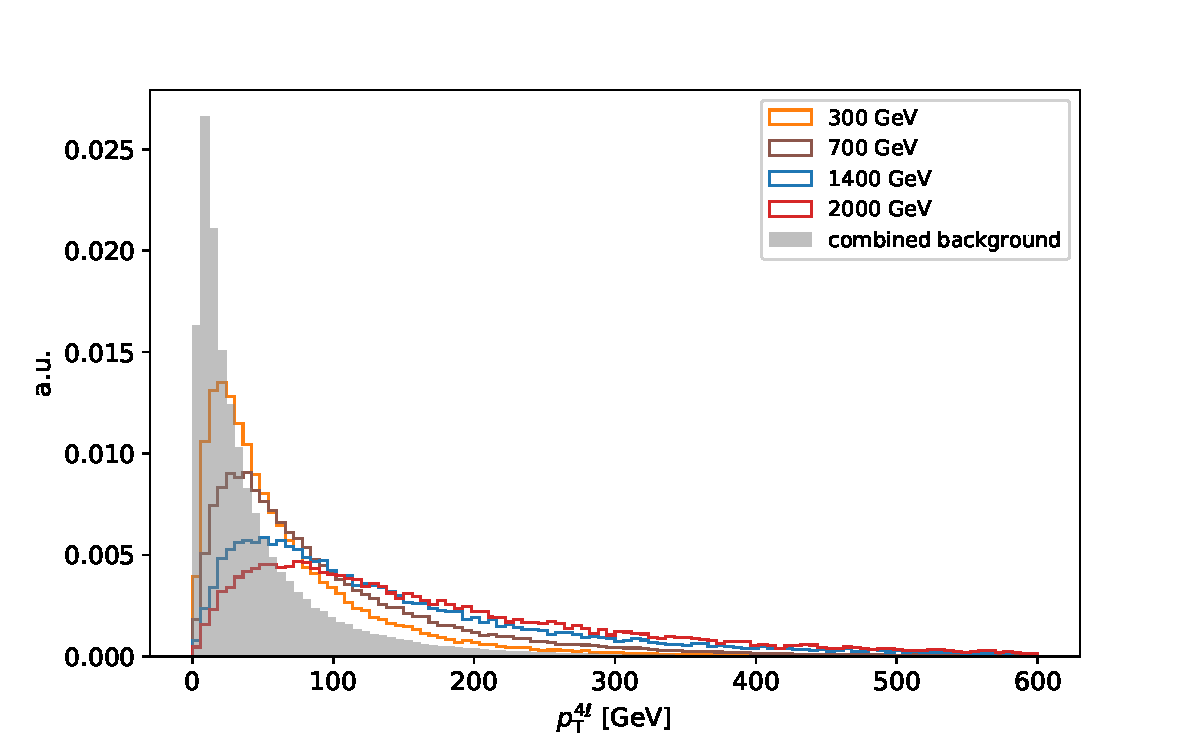
\includegraphics[width=0.24\textwidth]{figures/HMHZZ/selection/ggf_input/input_comparison_300_to_2000_11_score_pt4l_unconstrained}}
%        \subfloat[]{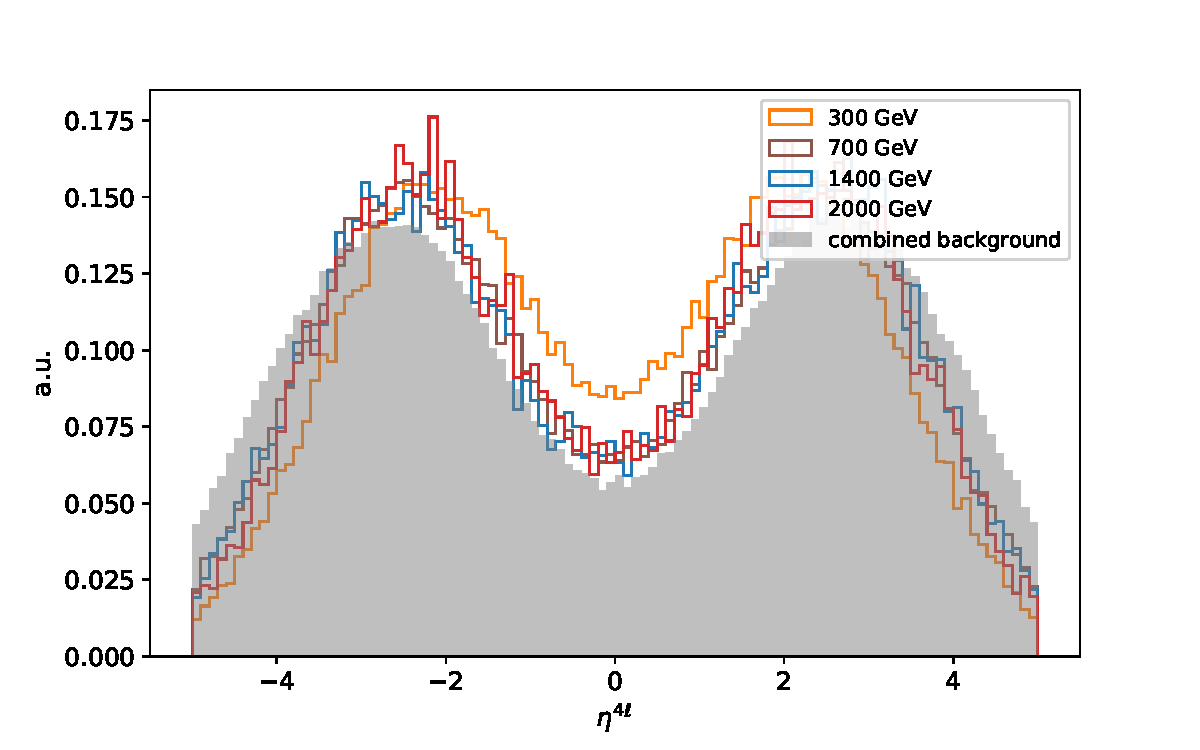
\includegraphics[width=0.24\textwidth]{figures/HMHZZ/selection/ggf_input/input_comparison_300_to_2000_12_score_eta4l_unconstrained}}\\
%
%        \subfloat[]{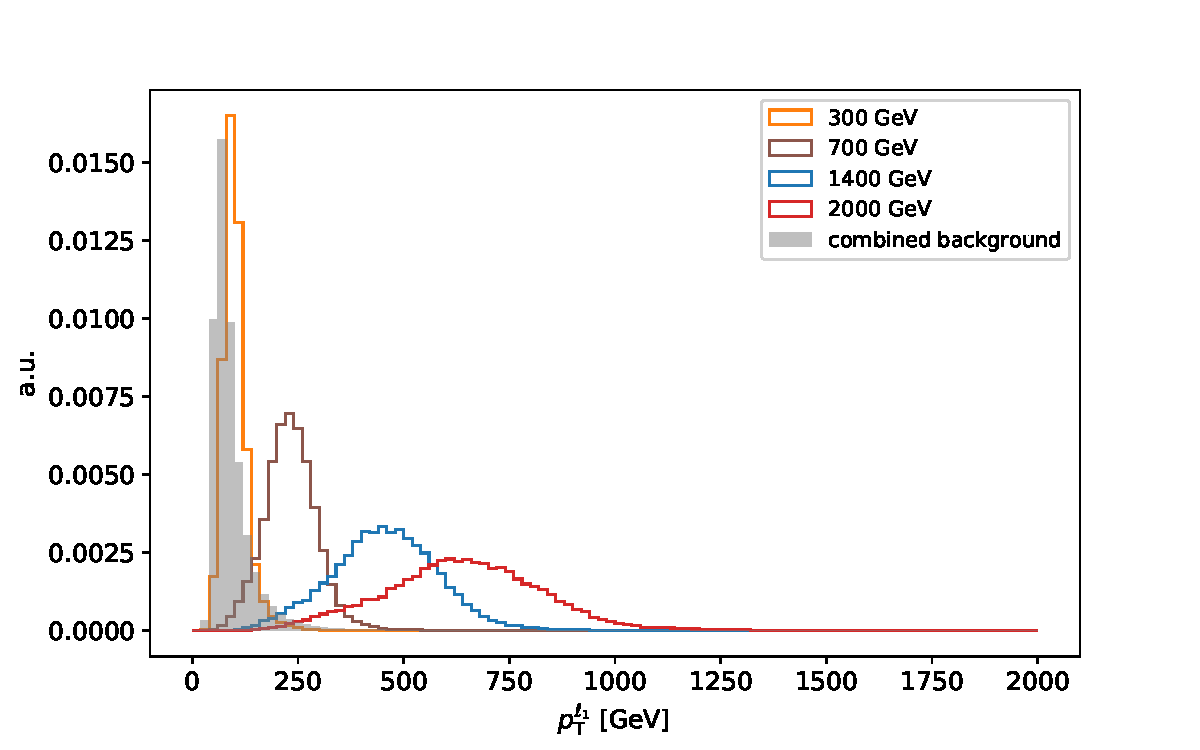
\includegraphics[width=0.24\textwidth]{figures/HMHZZ/selection/ggf_input/input_comparison_300_to_2000_15_score_lep_1_pt}}
%        \subfloat[]{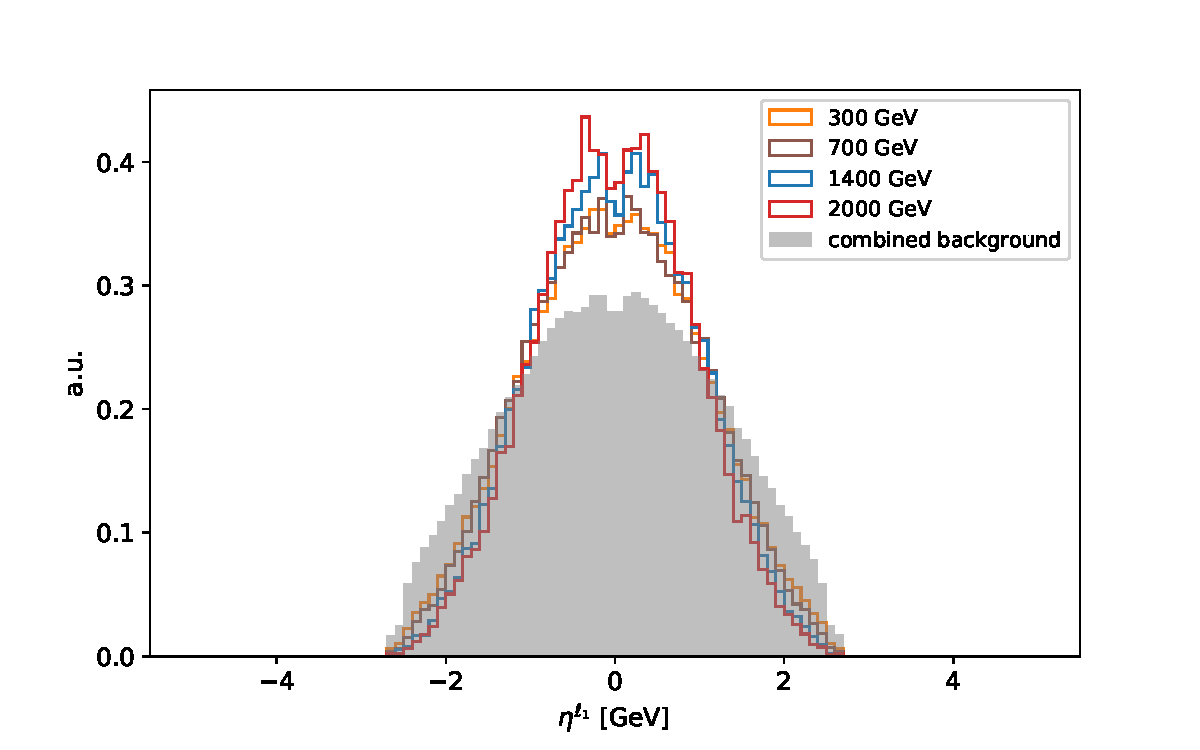
\includegraphics[width=0.24\textwidth]{figures/HMHZZ/selection/ggf_input/input_comparison_300_to_2000_16_score_lep_1_eta}}
%        \subfloat[]{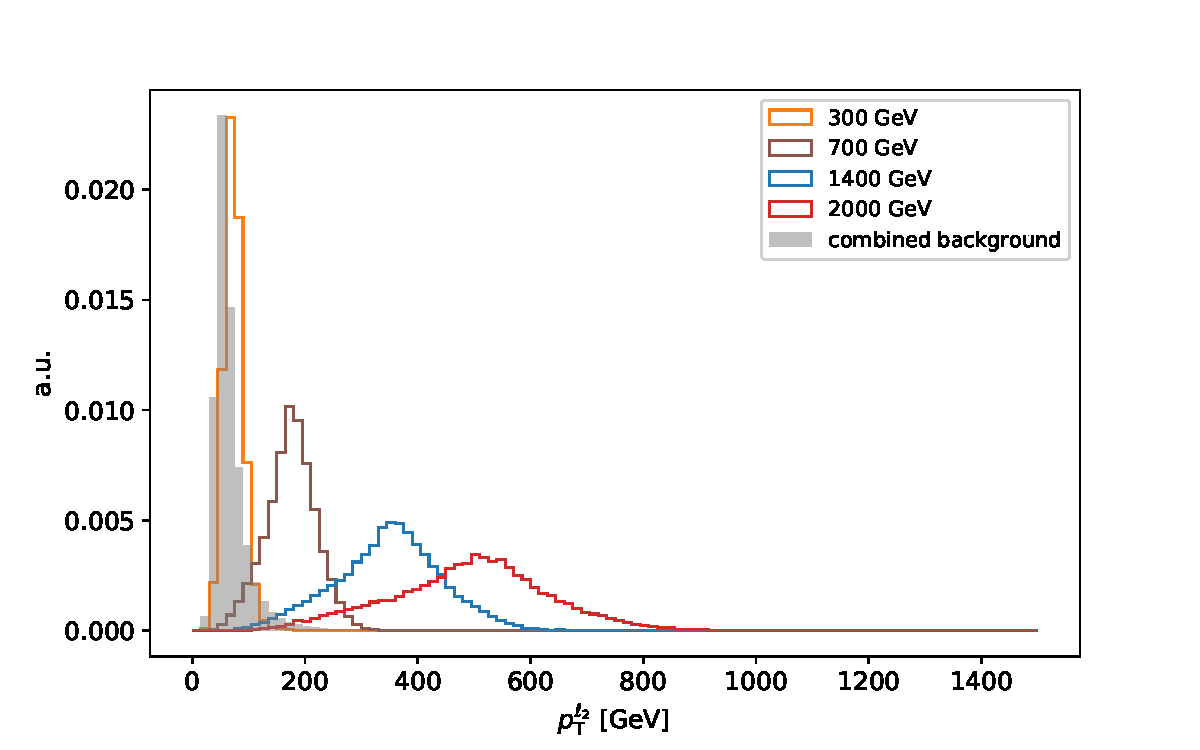
\includegraphics[width=0.24\textwidth]{figures/HMHZZ/selection/ggf_input/input_comparison_300_to_2000_17_score_lep_2_pt}}
%        \subfloat[]{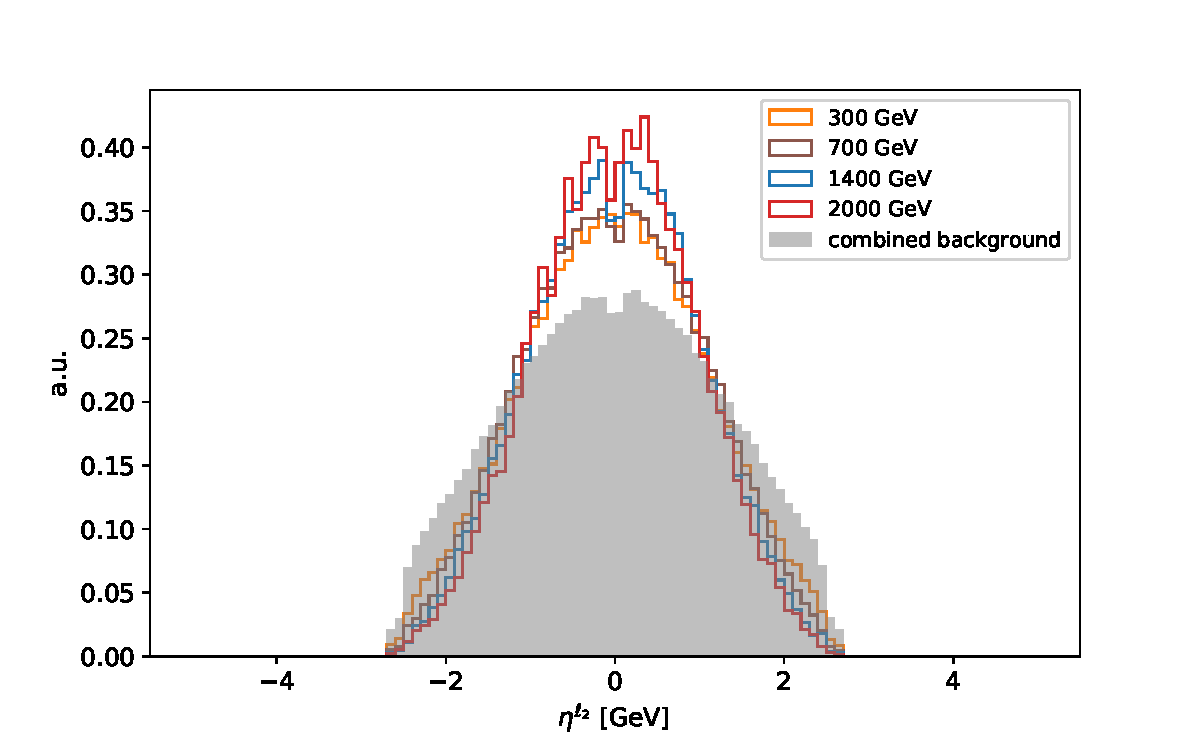
\includegraphics[width=0.24\textwidth]{figures/HMHZZ/selection/ggf_input/input_comparison_300_to_2000_18_score_lep_2_eta}}\\
%
%        \subfloat[]{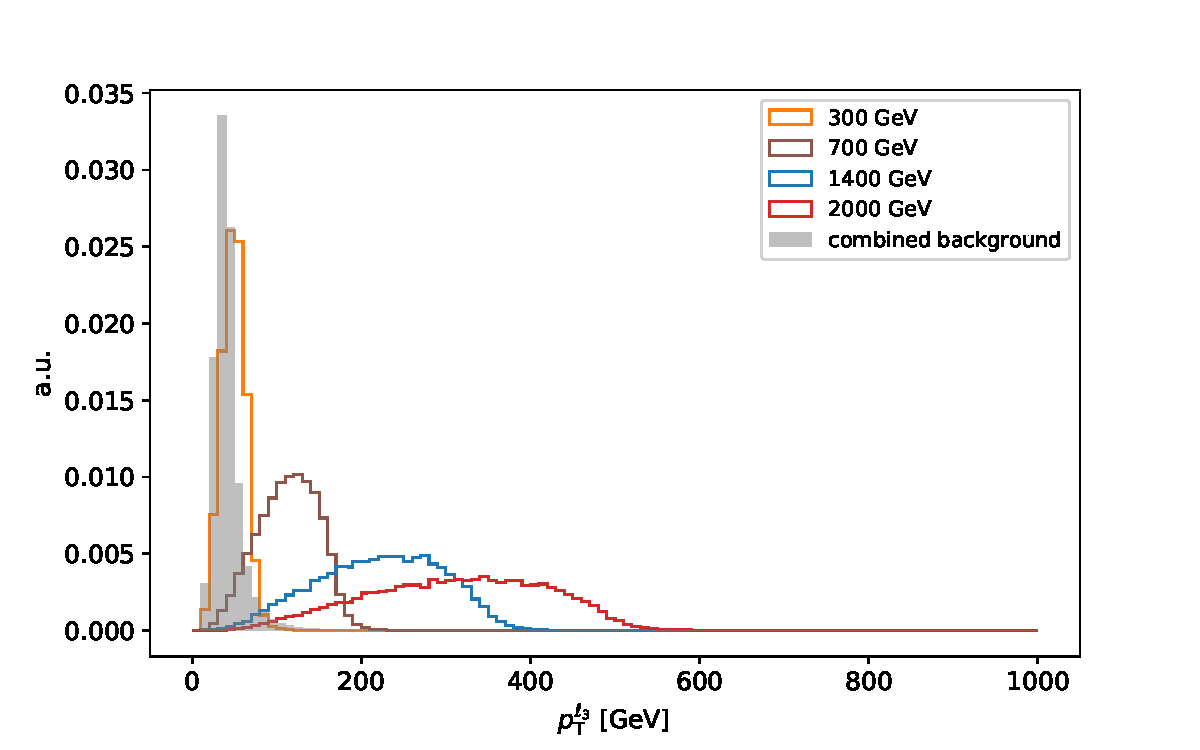
\includegraphics[width=0.24\textwidth]{figures/HMHZZ/selection/ggf_input/input_comparison_300_to_2000_19_score_lep_3_pt}}
%        \subfloat[]{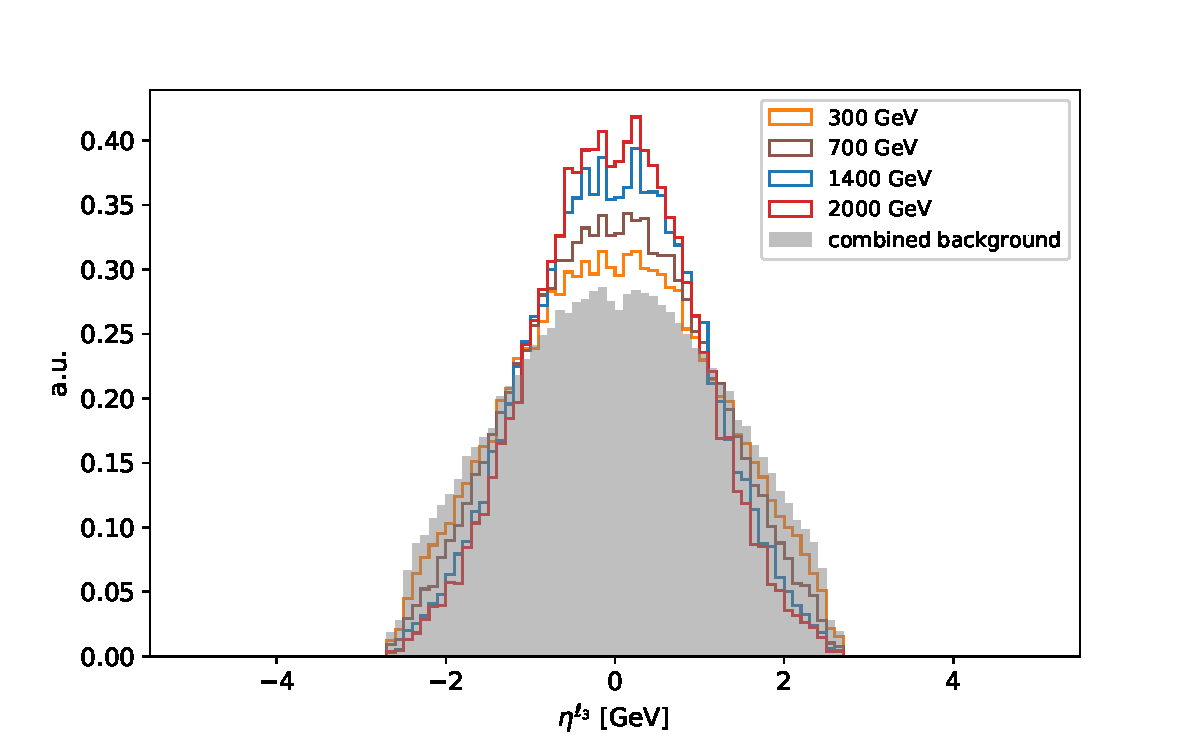
\includegraphics[width=0.24\textwidth]{figures/HMHZZ/selection/ggf_input/input_comparison_300_to_2000_20_score_lep_3_eta}}
%        \subfloat[]{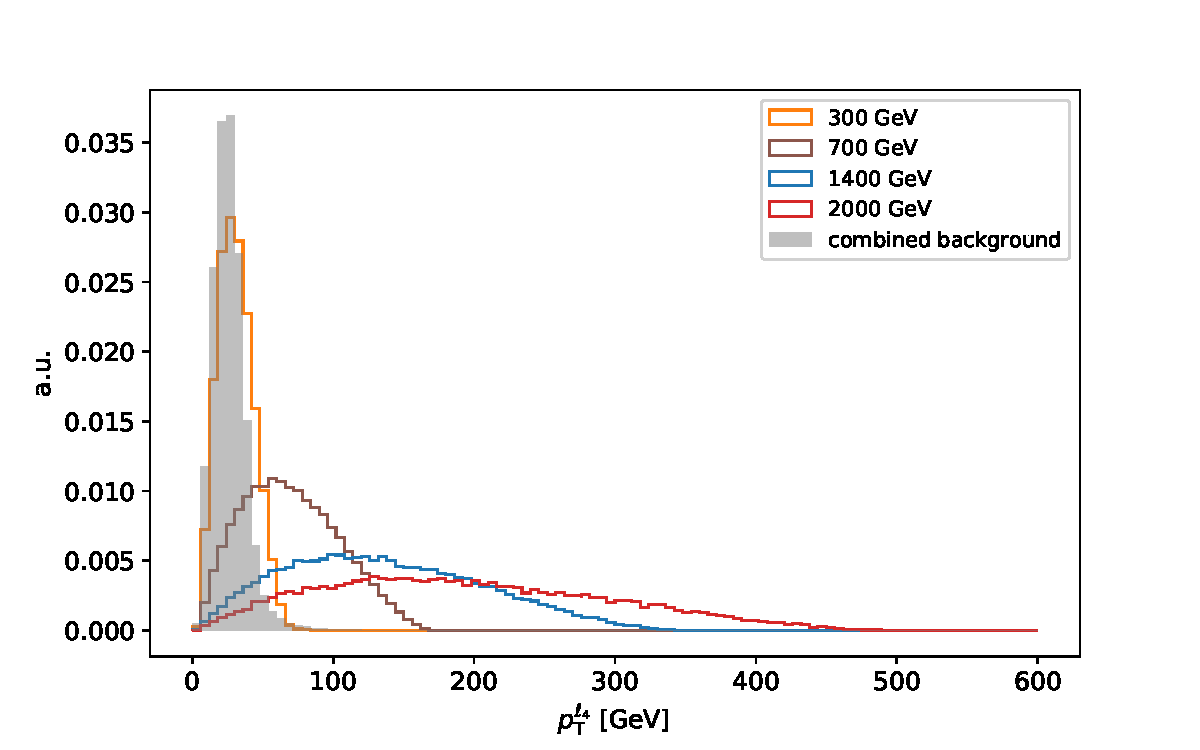
\includegraphics[width=0.24\textwidth]{figures/HMHZZ/selection/ggf_input/input_comparison_300_to_2000_21_score_lep_4_pt}}
%        \subfloat[]{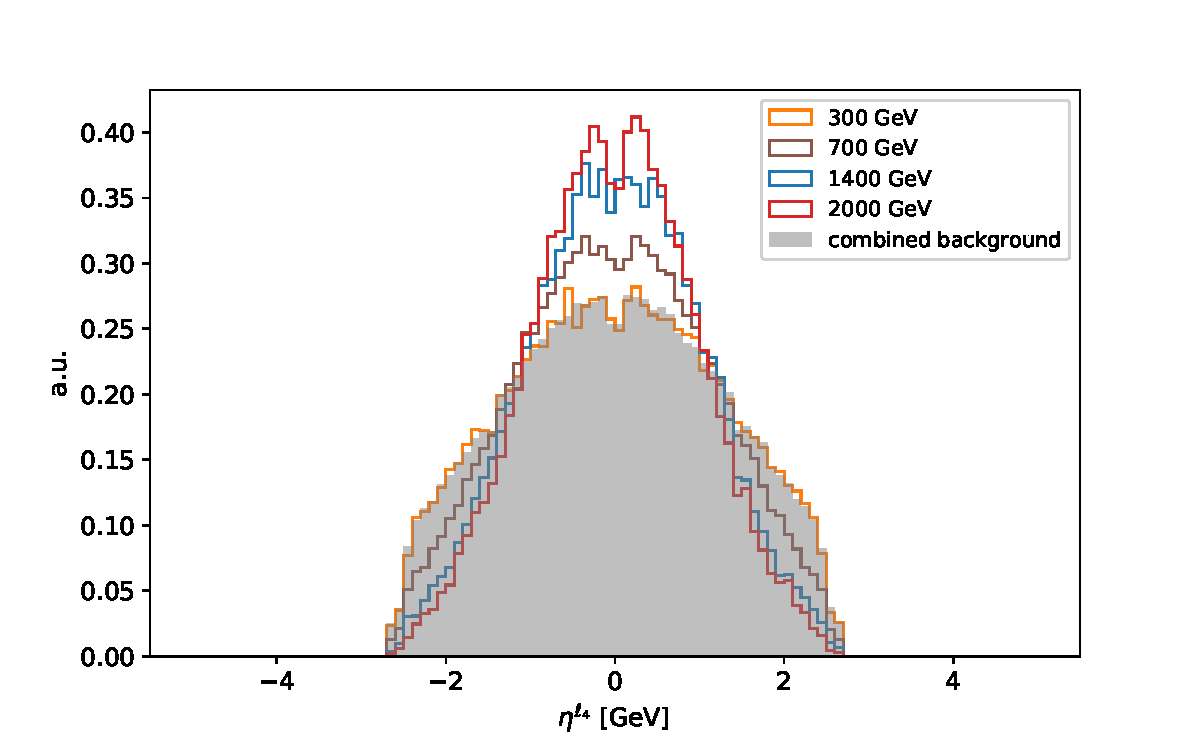
\includegraphics[width=0.24\textwidth]{figures/HMHZZ/selection/ggf_input/input_comparison_300_to_2000_22_score_lep_4_eta}}\\
%
%        \caption{Distributions of input features as listed in table~\ref{tab:dnn_features_ggf} for the ggF network of signals at mass points of 300, 700, 1400, 2000~\gev (coloured) and the background (grey). Events with any jet multiplicity are shown, as this model is evaluated in both $N_\mathrm{jets}\geq2$ and $N_\mathrm{jets}<2$.}
%        \label{fig:dnn_ggf_distribution}
%\end{figure}

\textbf{Evaluation of models} \\
Figure~\ref{fig:dnn_output_score} shows the classifier response output of background samples (QCD and EW \qqZZ and \ggZZ) as well as VBF (left) and ggF (right) signal sample at 700~\gev.

\begin{figure}[htbp]
        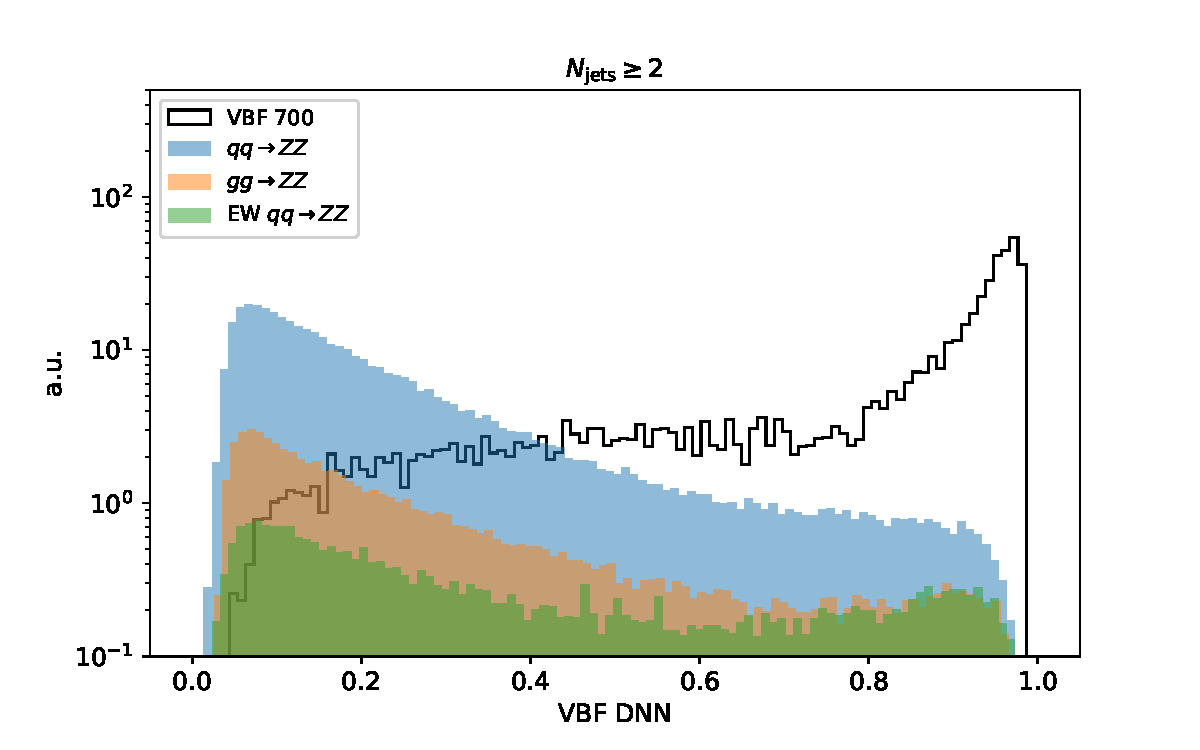
\includegraphics[width=0.48\textwidth]{figures/HMHZZ/selection/vbf_input/clf_output.pdf}
        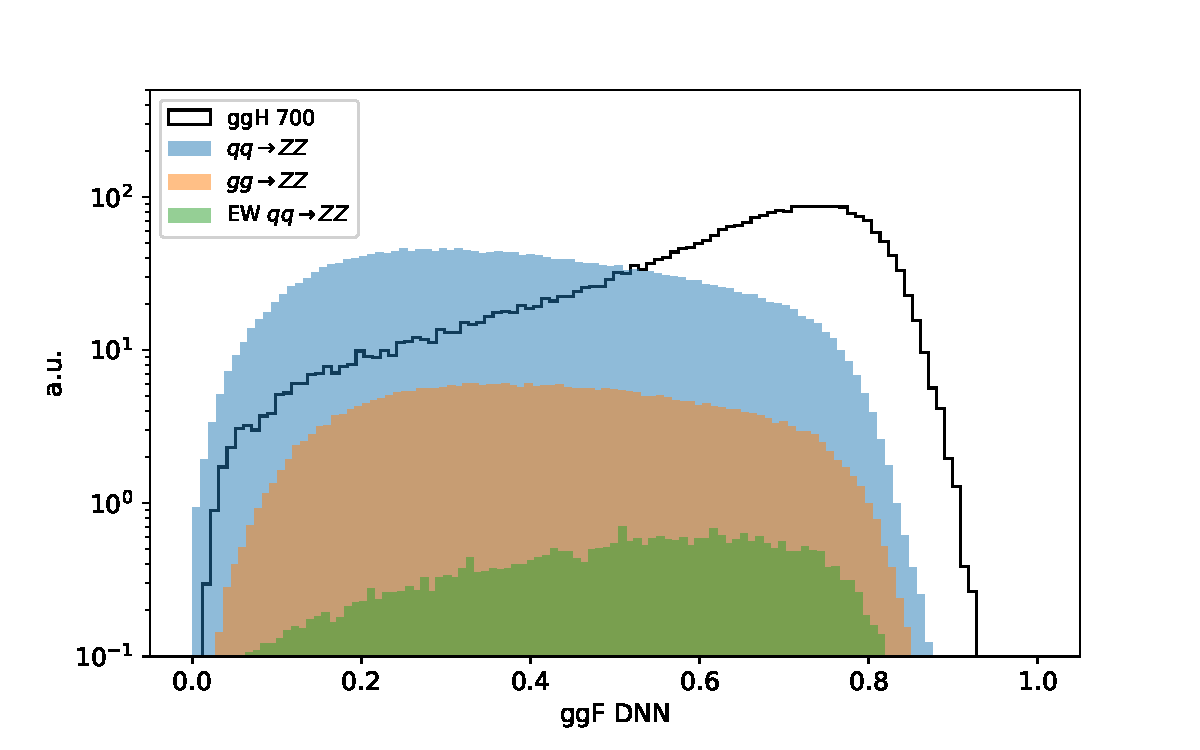
\includegraphics[width=0.48\textwidth]{figures/HMHZZ/selection/ggf_input/clf_output.pdf}
        \centering
        \caption{VBF (left) and ggF (right) output of the background samples (filled) and the $700~\gev$ signal sample (black).}
        \label{fig:dnn_output_score}
\end{figure}

Then the optimal cut at DNN output score is chosen based on an overall good performance of classifier to have a large significance improvement while retaining a high signal efficiency.
Figure~\ref{fig:dnn_significance} shows the significance improvements of DNN-based cuts when comparing with cut-based one at different VBF (left) and ggF (right) mass samples,
where the significance is calculated as:
\begin{equation}
Z = \sqrt{2\left(n\ln \left[ \frac{nb+\sigma^2}{b^2+n\sigma^2}\right]
        - \frac{b^2}{\sigma^2}\ln\left[1+\frac{\sigma^2(n-b)}{b(b+\sigma^2)}\right]\right)}
\end{equation}
Cut at 0.5 (0.8) for VBF (ggF) classifier is chosen as shown in solid lines.

\begin{figure}[htbp]
        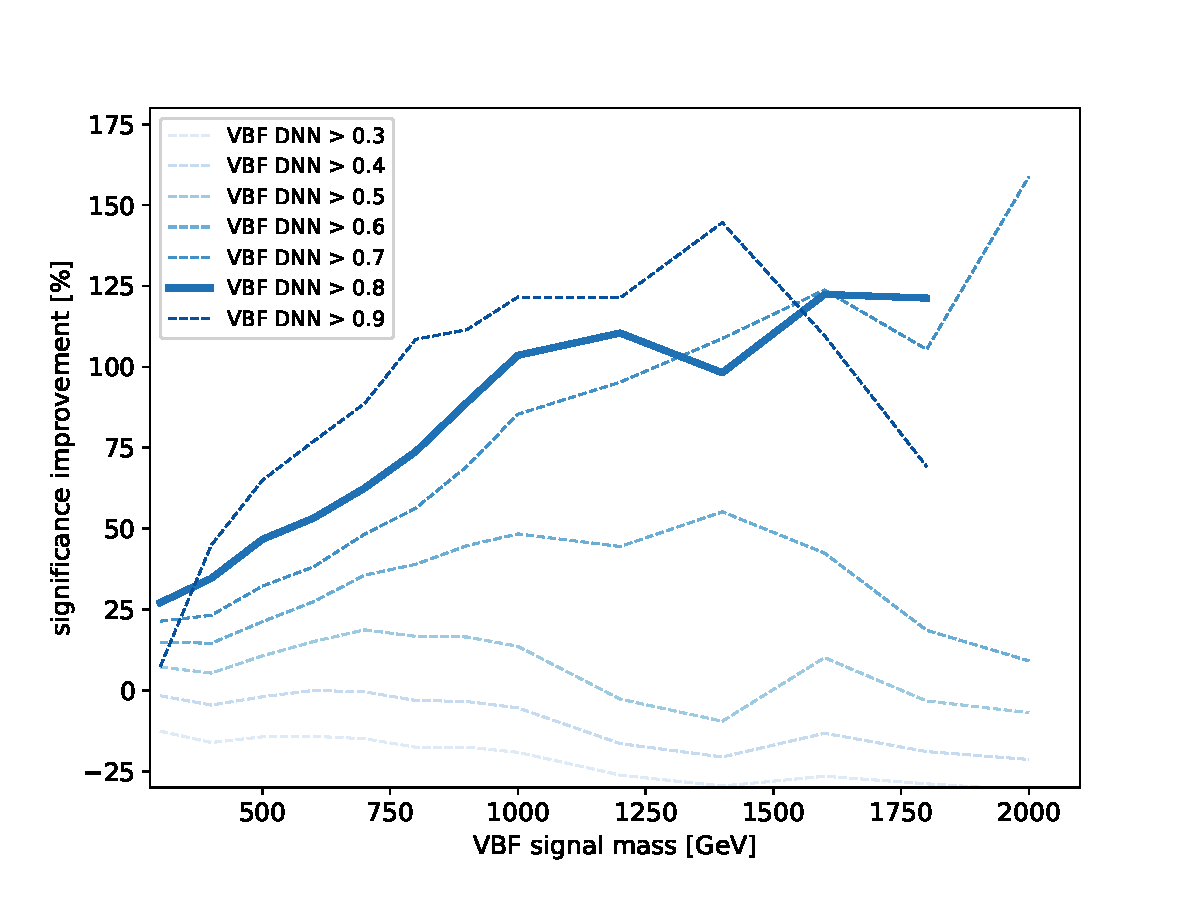
\includegraphics[width=0.48\textwidth]{figures/HMHZZ/selection/VBF_significance_improvement.pdf}
        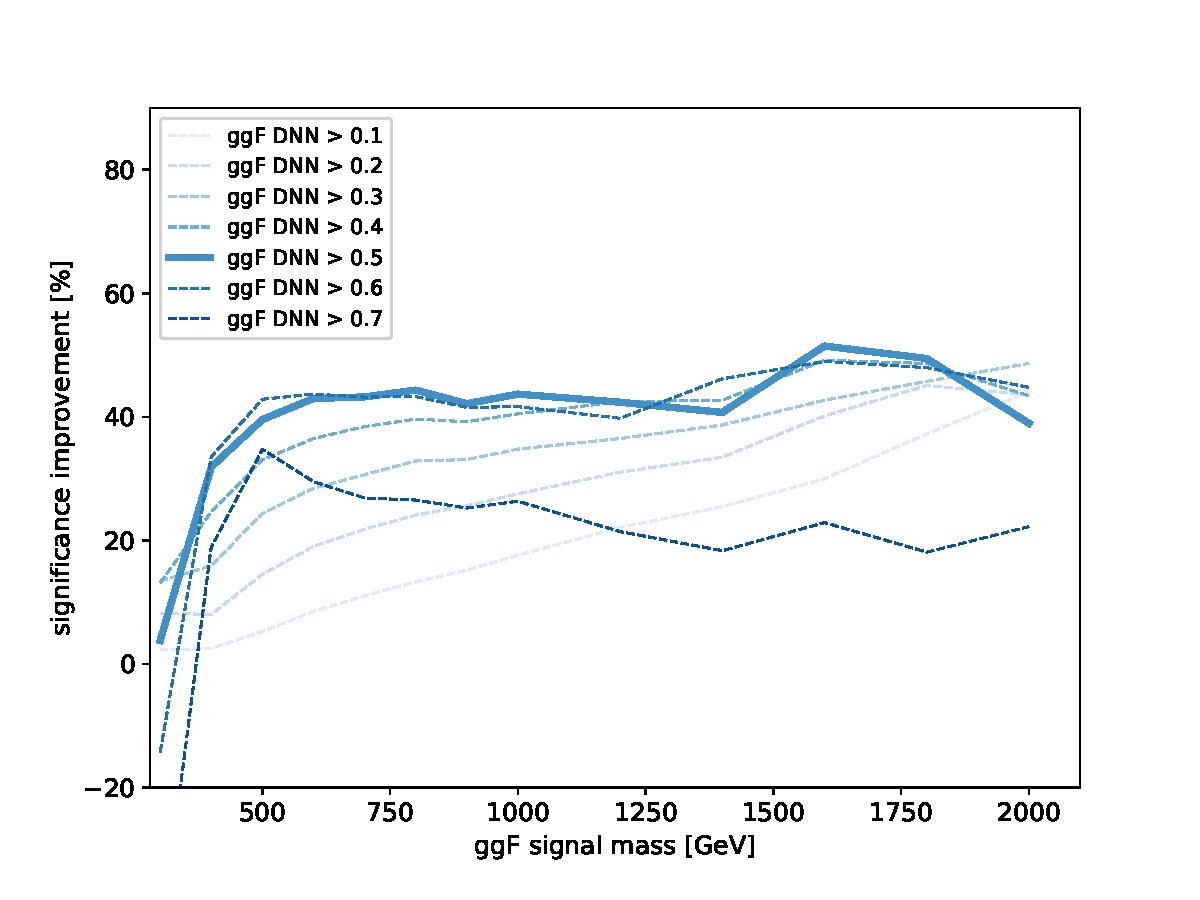
\includegraphics[width=0.48\textwidth]{figures/HMHZZ/selection/ggf_significance_improvement.pdf}
        \centering
        \caption{Significance improvements of the DNN-based over the cut-based categorization of the VBF (ggF) category for VBF (ggF) signal samples between 300 and 2000~\gev for seven different cuts on the VBF (ggF) DNN score. 
	The optimal cut of 0.8 (0.5) for VBF (ggF) DNN is chosen by a solid line, while other alternative cuts are plotted with dashed lines. 
	For VBF category, results at 2000~\gev for cuts of 0.8 and 0.9 are missing due to a lack of background events passing this tight selection.}
        \label{fig:dnn_significance}
\end{figure}

Then the events passing VBF classifier are categorized into VBF-enriched category.
Otherwise, the events failing VBF classifier but passing ggF classifier are categorized into ggF-enriched category, which is further split into 3 channels.
All remaining events are sorted into one additional category called 'rest'.
Thus there are five categories defined in DNN-based categorization, named: VBF, ggF\_2$e$2$\mu$, ggF\_4$e$, ggF\_4$\mu$ and rest.
In summary, cuts applied in categorization are defined as follow, and these phase spaces are also illustrated in figure~\ref{fig:hmhzz_dnncate}.

\begin{itemize}
	\item VBF-enriched category: Events have at least two selected jets ($\Njets \geq 2$), and with \DNNVBF > 0.8;
	\item ggF-enriched categories: $(\Njets \geq 2 \:\&\&\: \DNNVBF \leq 0.8 \:\&\&\: \DNNggF > 0.5) \:||\: (\Njets < 2 \:\&\&\: \DNNggF > 0.5)$; 
	\item rest category: All remaining events that fail VBF and ggF cuts mentioned above.
\end{itemize}

\begin{figure}[h]
\centering
\subfloat[]{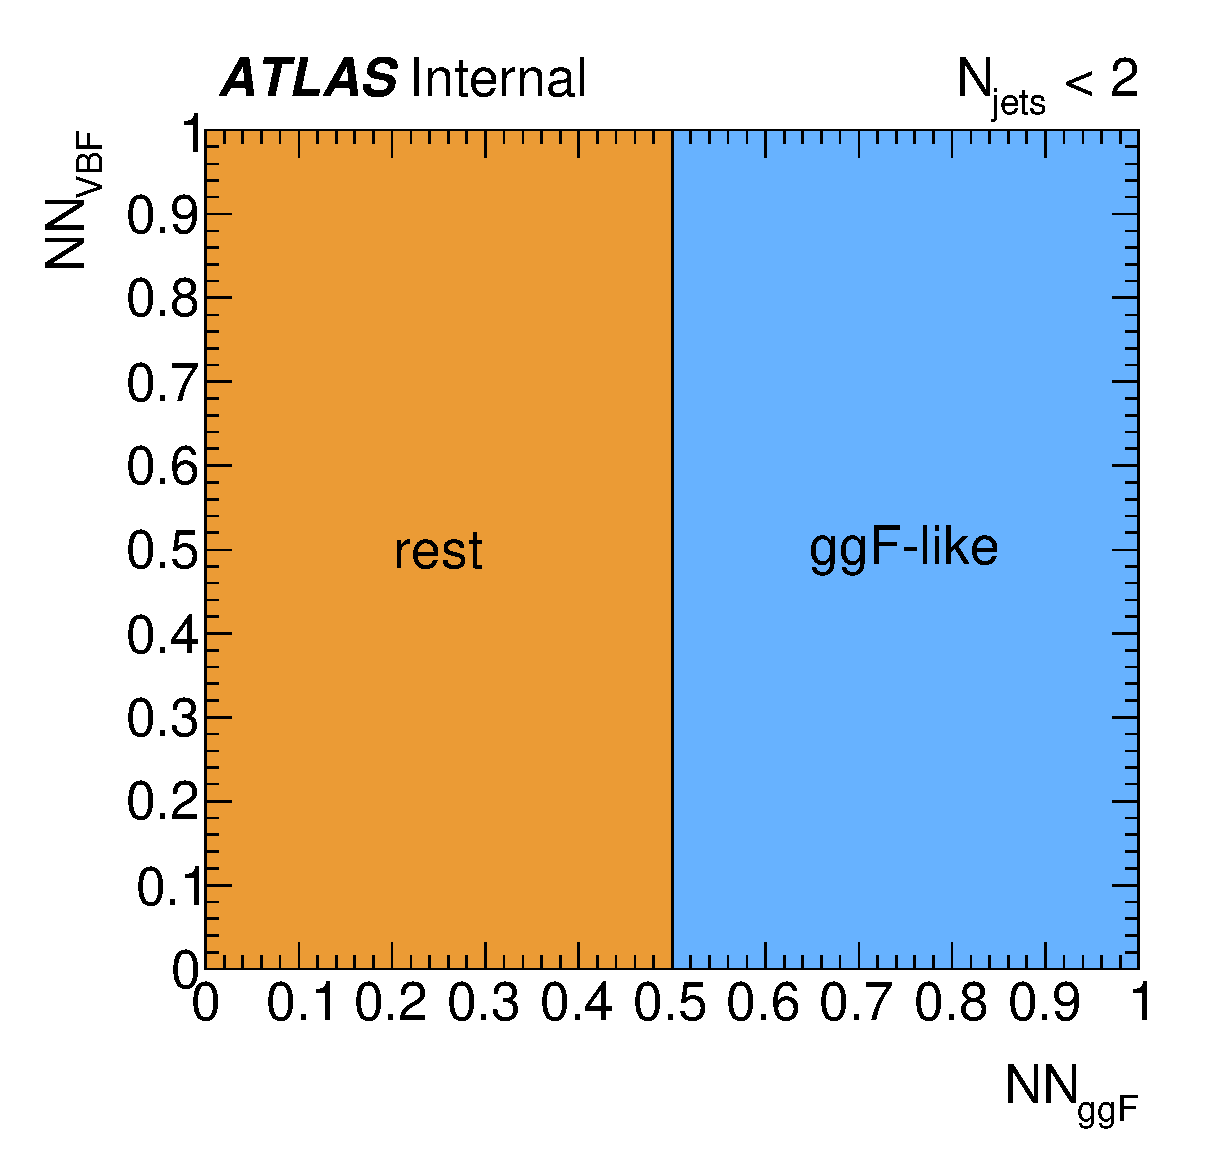
\includegraphics[width=0.43\textwidth]{figures/HMHZZ/selection/classifier_diagram_c1_njets_lt2.eps}}
\subfloat[]{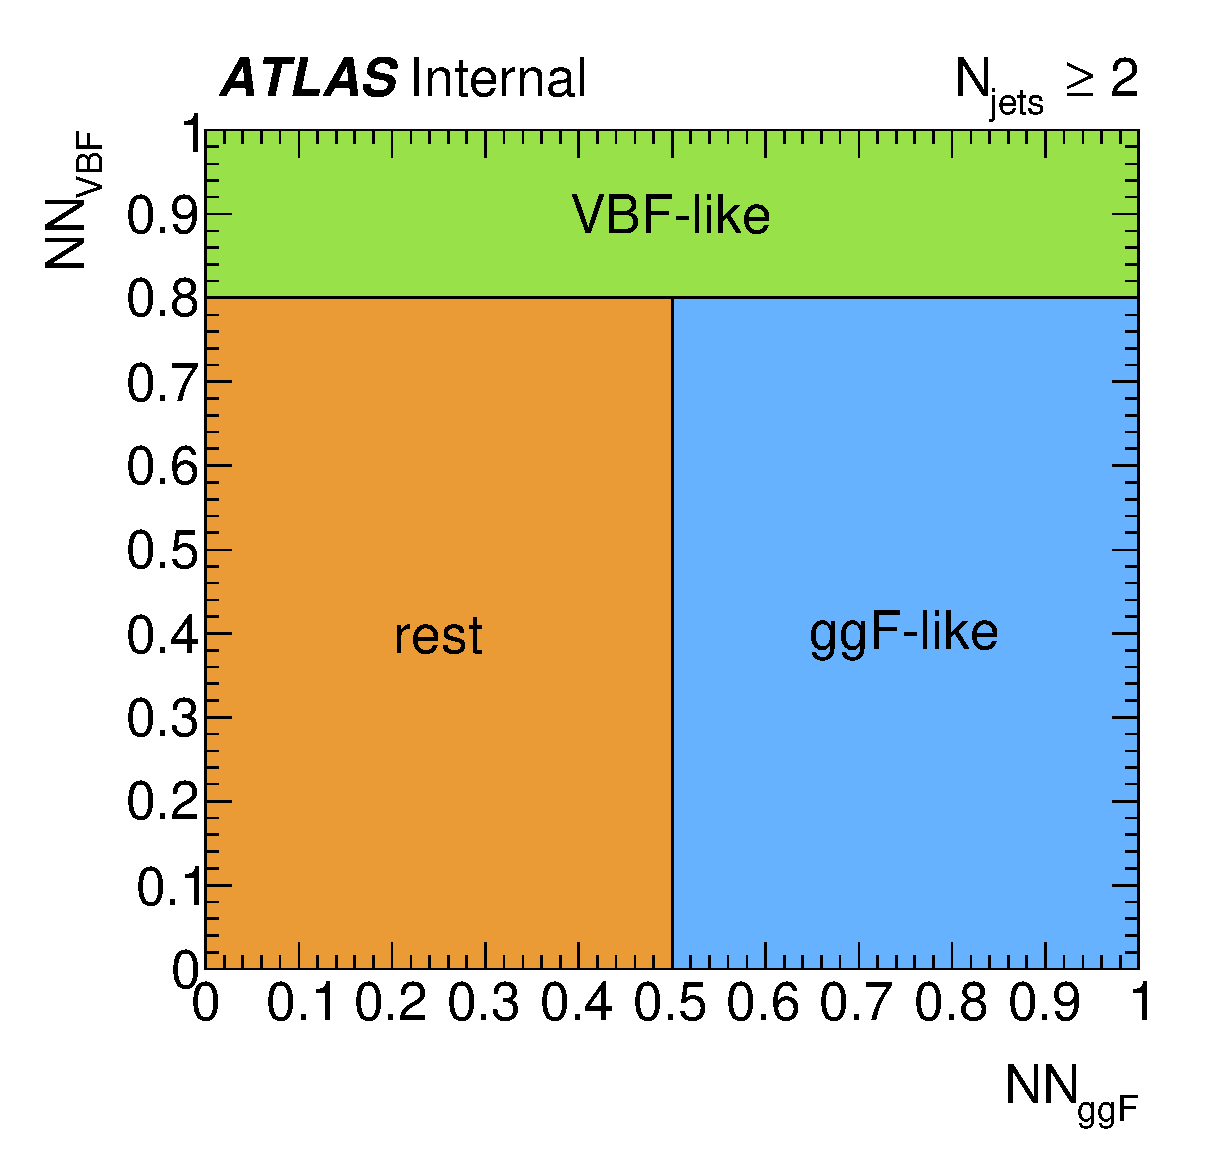
\includegraphics[width=0.43\textwidth]{figures/HMHZZ/selection/classifier_diagram_c1_njets_gt2.eps}}\\
\caption{Illustration of the DNN-based VBF and ggF event classification for events with (a) $\Njets < 2$ and (b) $\Njets \geq 2$.}
\label{fig:hmhzz_dnncate}
\end{figure}

\subsection{Signal acceptance} 
\label{sec:hmhzz_signal_acc}
The signal acceptance is defined as the ratio of events passing all analysis selection in each category to the total number of simulated events in whole phase space.
In denominator, the events with $\tau$ final states are not token into account.
And the contribution of $\tau$-lepton decay to electrons and muons final states is found to be negligible.

Figure~\ref{fig:hmhzz_acc_dnn} and ~\ref{fig:hmhzz_acc_cut} show the acceptance of NWA signal in DNN- and Cut- based categorization, estimated by merging the three signal MC campaigns, mc16a, mc16d and mc16e.
A 3-rd order polynomial fit is applied for each category.

\begin{figure}[h]
\centering
\subfloat[]{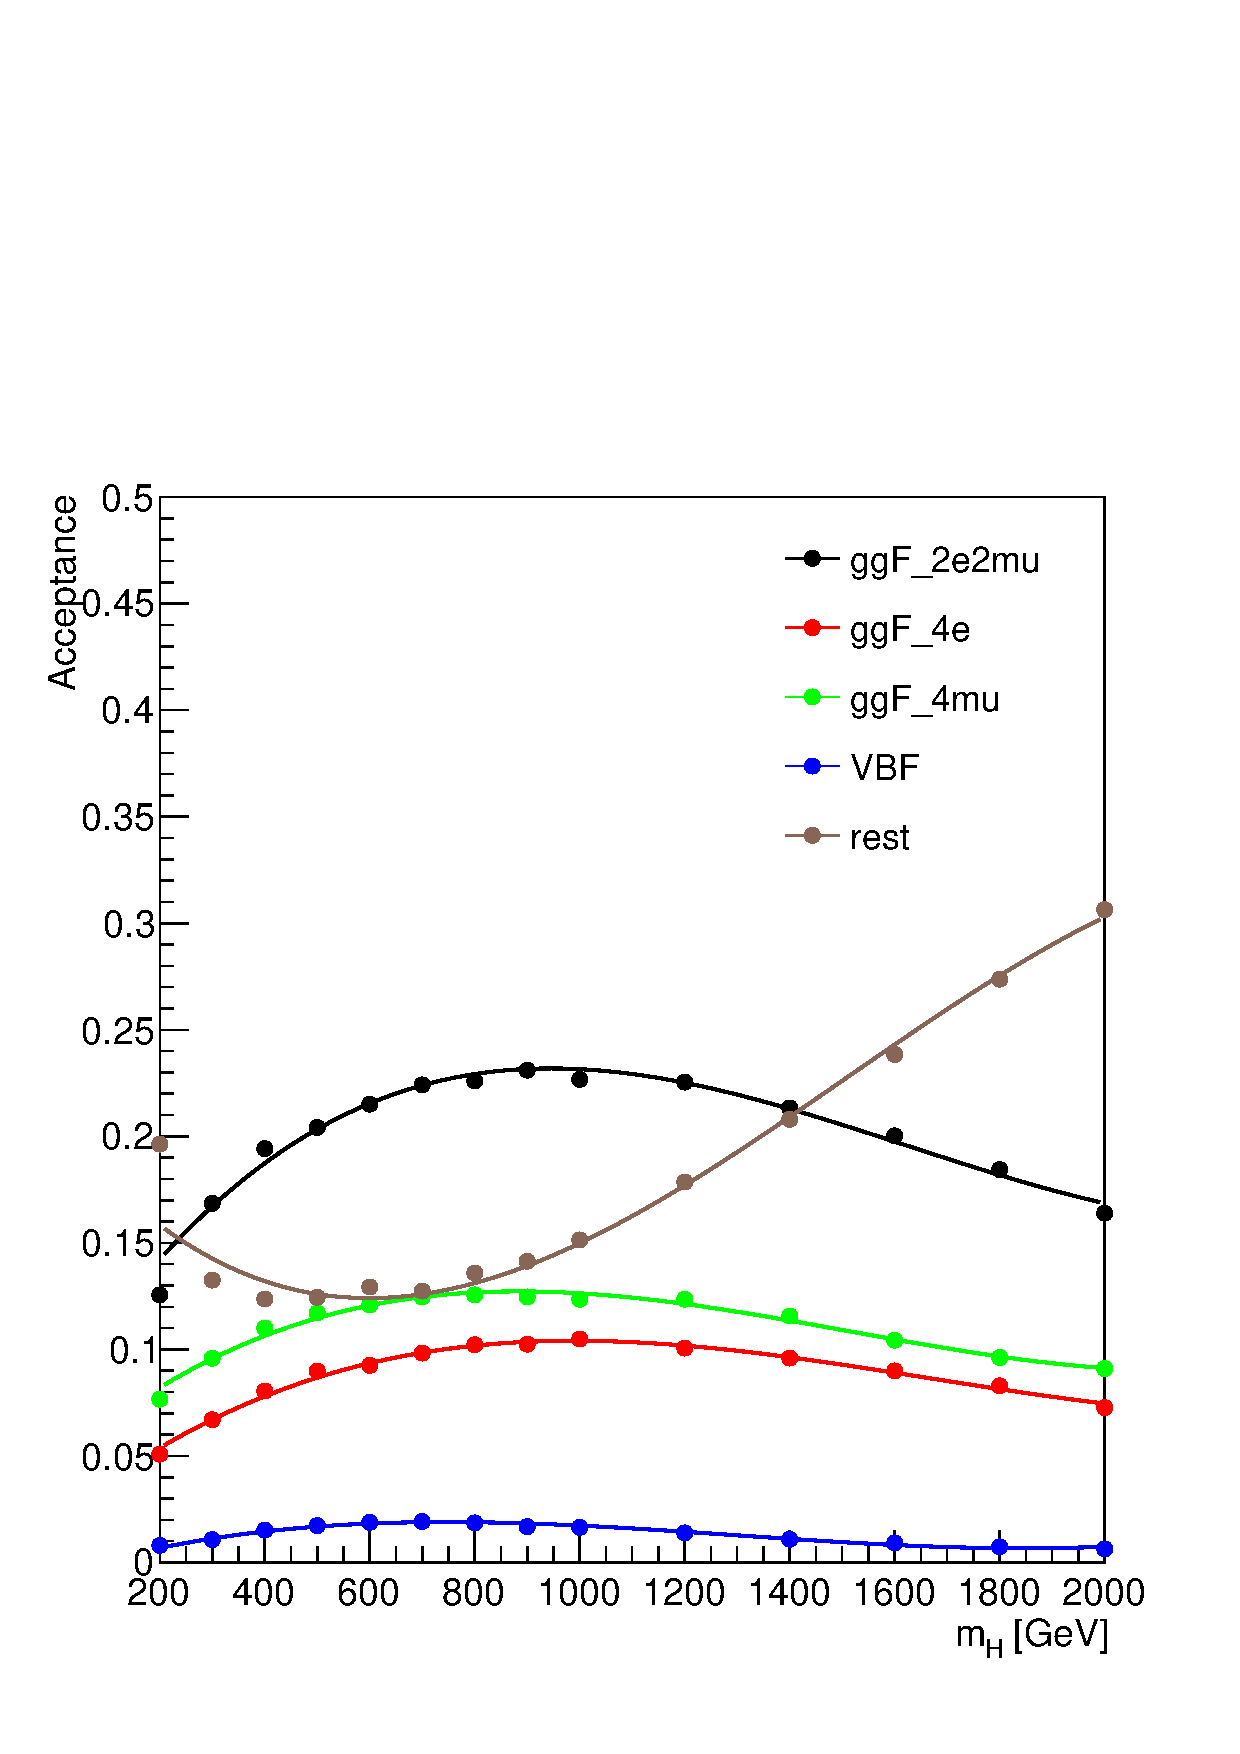
\includegraphics[width=0.43\textwidth]{figures/HMHZZ/selection/acc_dnn_ggF.pdf}}
\subfloat[]{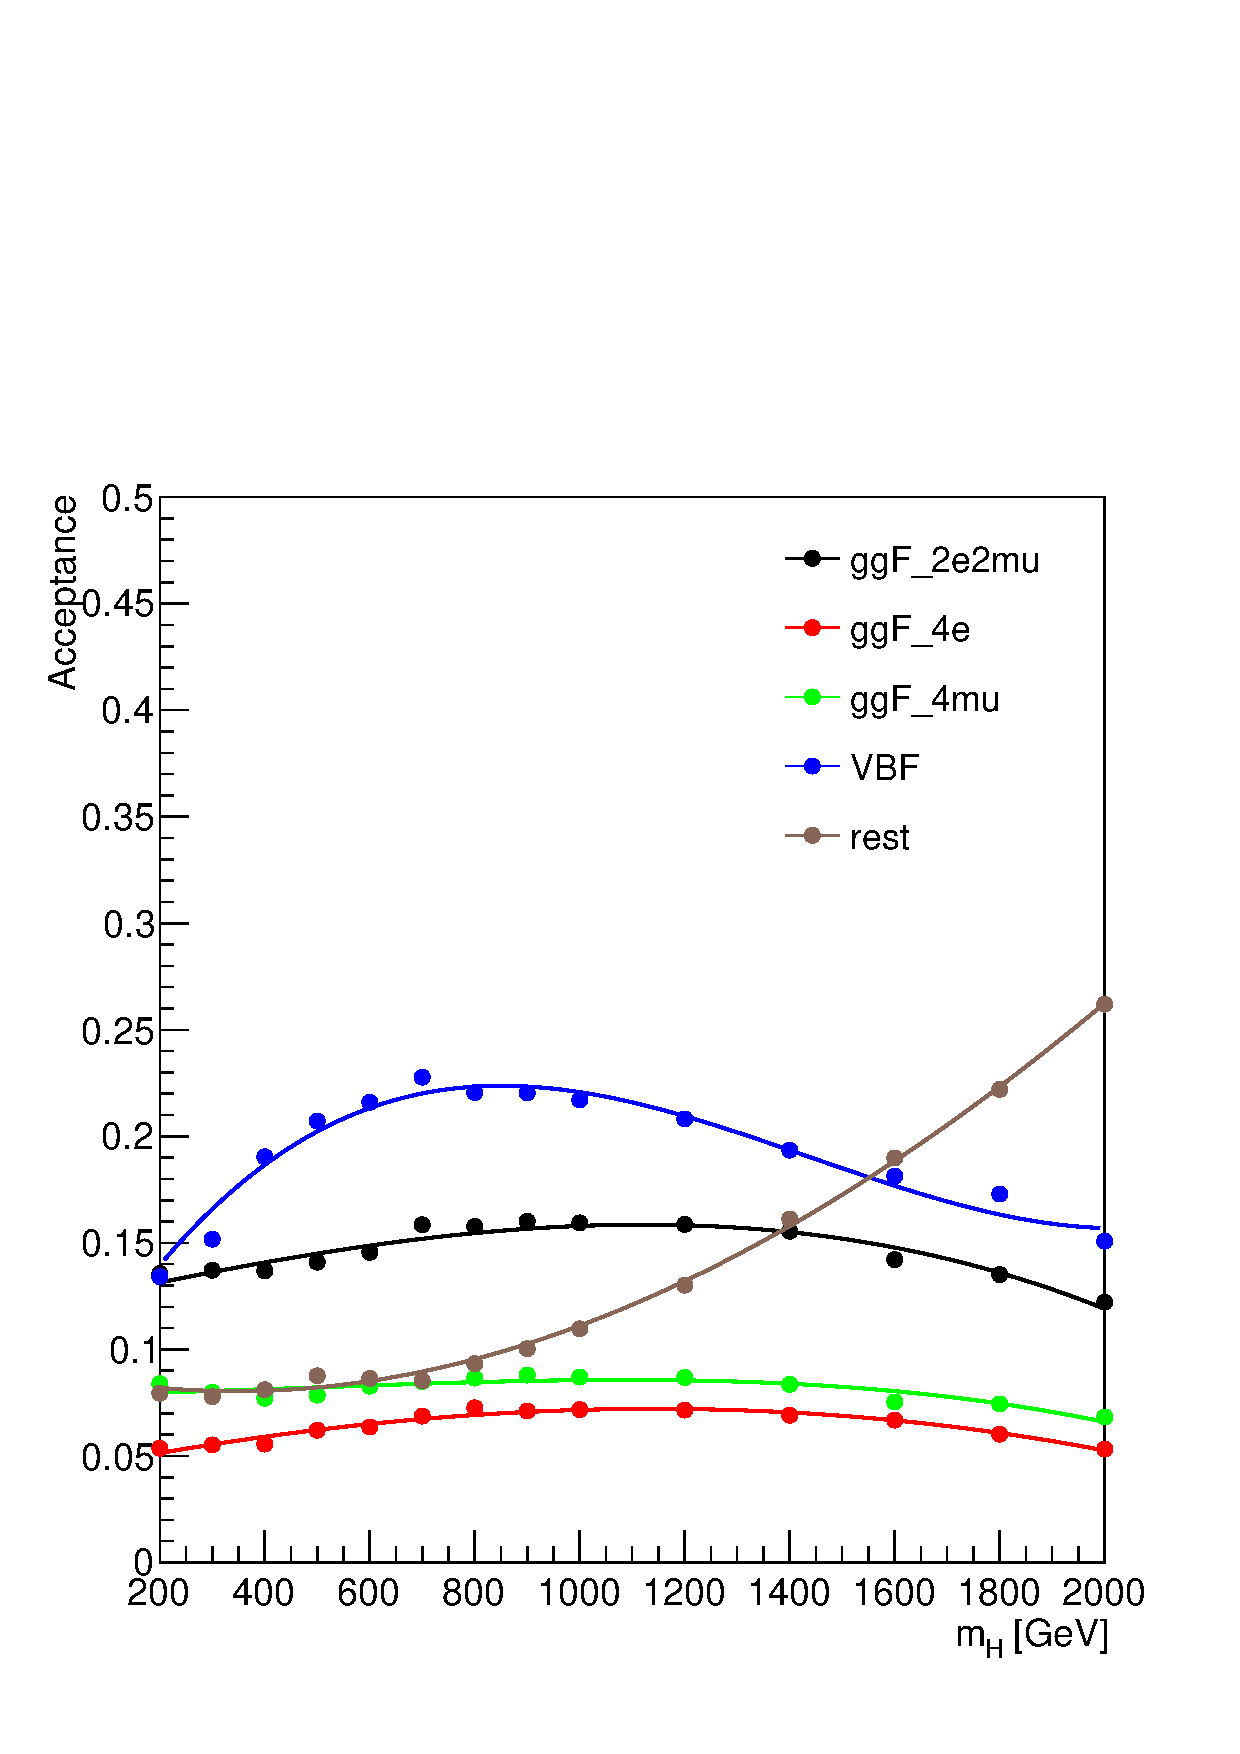
\includegraphics[width=0.43\textwidth]{figures/HMHZZ/selection/acc_dnn_VBF.pdf}}\\
\caption{NWA acceptance as a function of $m_{H}$ for the DNN-based categorization for the samples of
(a) ggF production mode;
(b) VBF production mode. 
}
\label{fig:hmhzz_acc_dnn}
\end{figure}

\begin{figure}[h]
\centering
\subfloat[]{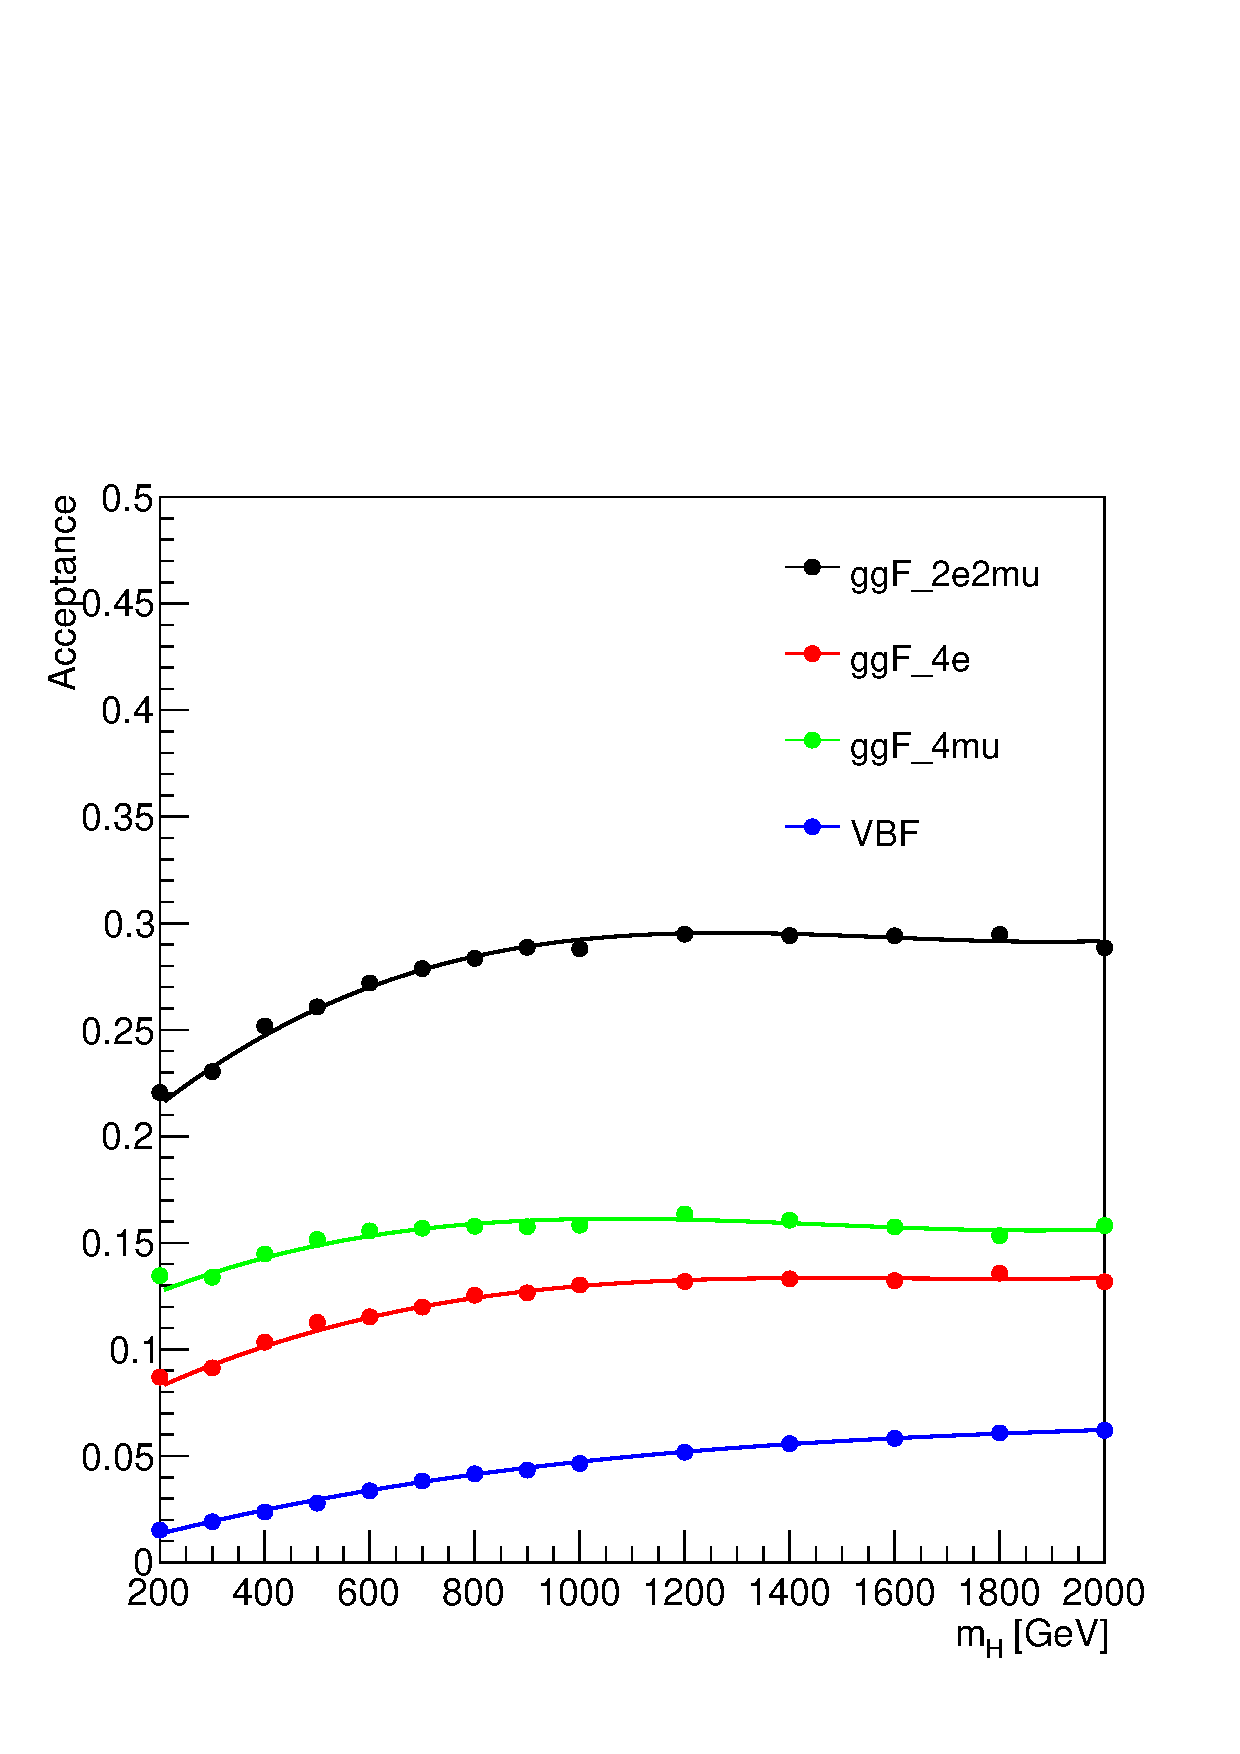
\includegraphics[width=0.43\textwidth]{figures/HMHZZ/selection/acc_cut_ggF.pdf}}
\subfloat[]{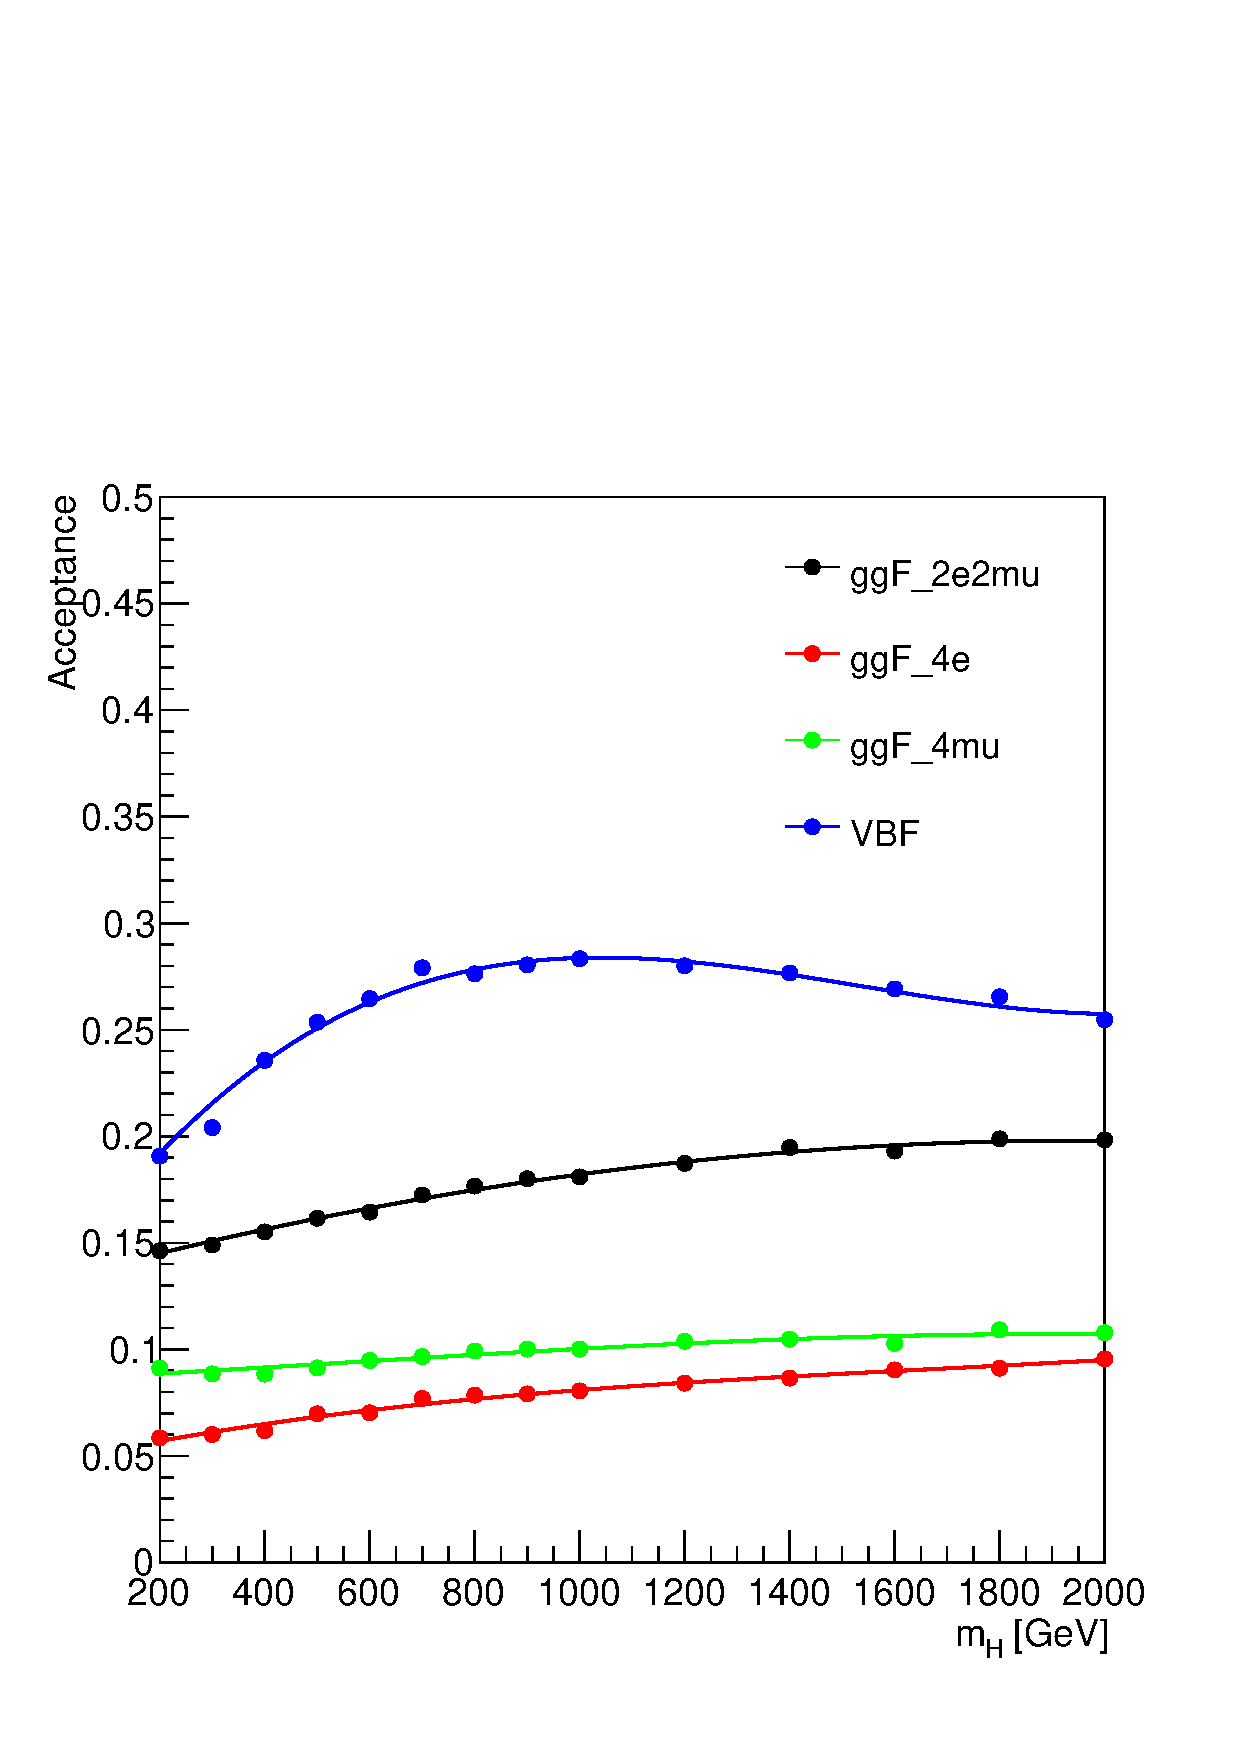
\includegraphics[width=0.43\textwidth]{figures/HMHZZ/selection/acc_cut_VBF.pdf}}\\
\caption{NWA acceptance as a function of $m_{H}$ for the Cut-based categorization for the samples of
(a) ggF production mode;
(b) VBF production mode. }
\label{fig:hmhzz_acc_cut}
\end{figure}
